%\documentclass[handout]{beamer} 
\documentclass[t,12pt,numbers,fleqn]{beamer}
%\documentclass[ignorenonframetext]{beamer}

\newif\ifquestions
%\questionstrue
\questionsfalse

\usepackage{pgfpages} 
\usepackage{hyperref}
\hypersetup{colorlinks=true,
    linkcolor=blue,
    citecolor=blue,
    filecolor=blue,
    urlcolor=blue,
    unicode=false}
\urlstyle{same}

\usepackage{tikz}
\usetikzlibrary{positioning}

\usepackage{booktabs}
\usepackage{listings}
\lstset{frame=none, showstringspaces=false, basicstyle=\ttfamily\bfseries\footnotesize,
  xleftmargin=-8mm,language=Haskell,breaklines=true}

\newcommand{\colAwidth}{0.1\textwidth}
\newcommand{\colBwidth}{0.8\textwidth}

\renewcommand{\arraystretch}{1.1} %so that tables with equations do not look crowded

\usepackage{pifont}
\usepackage{amsmath,amsfonts,xspace,xcolor,url}
\newcommand{\cross}{\ding{55}}

\bibliographystyle{plain}

%\usetheme{Iimenau}

\useoutertheme{split} %so the footline can be seen, without needing pgfpages

%\pgfpagesuselayout{resize to}[letterpaper,border shrink=5mm,landscape]  %if this is uncommented, the hyperref links do not work

\mode<presentation>{}

\input{../def-beamer}

\newcommand{\topic}{21 Artifact Generation}

%Title page information for 1D04 lectures slides

% Define year specific parameters - used in title page and footer

\newcommand{\season}{Fall} %use to switch between Winter and Fall
\newcommand{\instructor}{Dr.~Spencer Smith} %use to switch instructor
\newcommand{\instructSmall}{Dr.~Smith}
\newcommand{\yr}{2019}
\newcommand{\courseCode}{CAS 741, CES 741}
\newcommand{\courseTitle}{Development of Scientific Computing Software}

%\setbeamerfont{structure}{series=\bfseries}
%\usefonttheme[stillsansseriftext,stillsansserifmath]{serif}
\setbeamertemplate{navigation symbols}{} 
\setbeamertemplate{itemize item}[ball]

\title{
  {\normalsize \bf 
    \borange{\courseCode~(\courseTitle)\\ \season~\yr}}\\[2ex]
  {\Large \bf \topic}}

\author[Smith]{\instructor}

\institute{
  Faculty of Engineering,
  McMaster University}

\date{
\today
%January 2011\\
\bc
  \includegraphics[scale = 0.2, keepaspectratio]
  {../mcmaster-logo-full-color.jpg}
\ec
}

\renewcommand{\borange}[1] %orange is too hard to read
{
   \bred{#1}
}

\begin{document}

\input{../footline}

%%%%%%%%%%%%%%%%%%%%%%%%%%%%%%%%%%%%%%%%%%%%%%%%%%%%%%

\begin{frame}
\frametitle{Artifact Generation}

\bi
\item Administrative details
\item Next week's presentations
\item Feedback on VnV
\item Questions about MG/MIS?
\item Implementing an MIS 
\item Artifact generation (Drasil)
\ei
\end{frame}

%%%%%%%%%%%%%%%%%%%%%%%%%%%%%%%%%%%%%%%%%%%%%%%%%%%%%%

\begin{frame}
\frametitle{Administrative Details}

\bi
\item For final documentation, make sure you have \textbf{addressed and closed}
  all open issues
\item MIS marking scheme on Avenue
% \bi
% \item On Avenue
% \item Not all of the spec has to be formal
% \item First steps
% \bi
% \item Syntax of access programs
% \item State variables?
% \item Environment variables?
% \ei
% \ei
\item Course evaluation
\bi
\item Thurs, Nov 21, 10:00 am to Thurs, Dec 5, 11:59 pm
\item \url{https://evals.mcmaster.ca}
\ei
\item Module implementation
\bi
\item Assign to your domain expert the implementation of one module
\item Grading will be generous, as long as you make a concerted effort
\ei
\ei

\end{frame}

%%%%%%%%%%%%%%%%%%%%%%%%%%%%%%%%%%%%%%%%%%%%%%%%%%%%%%

\begin{frame}
\frametitle{Administrative Details: Report Deadlines}
~\newline
\begin{tabular}{l l l}
MG + MIS & Week 10 & Today!\\
Final Documentation & Week 14 & Dec 9\\
\end {tabular}

\bi
\item The written deliverables will be graded based on the repo contents as of
11:59 pm of the due date
\item If you need an extension, please ask
\item Two days after each major deliverable, your GitHub issues will be due
\item Domain expert code due 1 week after MIS deadline (after assigned issue by
  project owner)
\ei

\end{frame}

%%%%%%%%%%%%%%%%%%%%%%%%%%%%%%%%%%%%%%%%%%%%%%%%%%

\begin{frame}
\frametitle{Administrative Details: Presentations}

~\newline
\begin{tabular}{l l l}
Unit VnV or Impl.\ Present & Week 12 & Week of Nov 25\\
\end {tabular}

\bi
\item Informal presentations with the goal of improving everyone's written
  deliverables
\item Domain experts and secondary reviewers (and others) will ask questions
  (listed in Repos.xlsx file)
\ei

\end{frame}

%%%%%%%%%%%%%%%%%%%%%%%%%%%%%%%%%%%%%%%%%%%%%%%%%%

\begin{frame}
\frametitle{Administrative Details: Presentation Schedule}

\bi
\item Unit VnV Plan or Impl.\ Present
\bi
\item Monday: Bo, Sasha, ?
\item Thursday: Zhi, Peter, Ao
\ei
\ei

Optional presentation in italics.\\
Room for more volunteers.  :-)

\end{frame}

%%%%%%%%%%%%%%%%%%%%%%%%%%%%%%%%%%%%%%%%%%%%%%%%%%%%%%

\begin{frame}
\frametitle{Administrative Details: Unit VnV or Impl.\ Present}

Can present anything related to the implementation or testing
\bi
\item Code
\item Tools used
\item Testing
\item Unit VnV Plan
\item API documentation via doxygen
\item As always it is fine to show work in progress
\item Good to bring questions to the class
\ei

\end{frame}

%%%%%%%%%%%%%%%%%%%%%%%%%%%%%%%%%%%%%%%%%%%%%%%%%%%%%%

\begin{frame}
\frametitle{Feedback on VnV Plan}

\bi
\item Explicit web-link to your GitHub repo
\item Reference all your other documents (even the unwritten ones)
\item Explicitly state programming language
\item Very nice to have explicit cross-references between documents.  Keep
  information up to date using make
\item Do not postpone decisions, be specific
\item Outputs are unlikely to be an exact match for expected, instead summarize
  the error for all tests
\item Define what you mean by error, especially if the output is a sequence
\item Avoid unnecessary repetition, summarize similar tests in a table,
  distinguished by variabilities
\ei

\end{frame}

%%%%%%%%%%%%%%%%%%%%%%%%%%%%%%%%%%%%%%%%%%%%%%%%%%%%%%

\begin{frame}
\frametitle{VnV Feedback Continued}

\bi
\item Spell check!  Proof read!
\item Great to see usability tests% , but need more information on how tests will
  % be run.  For instance, what specific task will they be asked to perform?
\item Great to see code walkthroughs, but need more detail
\item Provide enough information that the reader can easily verify your test cases% ,
  % especially the expected output
\item \textbf{Write as if someone else will be doing the testing}
\ei

\end{frame}

%%%%%%%%%%%%%%%%%%%%%%%%%%%%%%%%%%%%%%%%%%%%%%%%%%%%%%

\begin{frame}
\frametitle{Questions?}
\begin{itemize}
\item Questions about MG/MIS
\end{itemize}
\end{frame}

%%%%%%%%%%%%%%%%%%%%%%%%%%%%%%%%%%%%%%%%%%%%%%%%%%%%%%

\begin{frame}
\frametitle{Implementing Your MIS}
\begin{itemize}
\item The mapping between the MIS and the code is generally not ``term'' by
  ``term''
\item You do not need to use the mathematical type listed in the spec
\item Consider A2 (Allocation to Engineering Programs)
\begin{itemize}
\item
  \href{https://gitlab.cas.mcmaster.ca/smiths/se2aa4_cs2me3/blob/master/Assignments/A2/A2.pdf}
  {Problem Description}
\item
  \href{https://gitlab.cas.mcmaster.ca/smiths/se2aa4_cs2me3/tree/master/Assignments/A2/A2Soln/src}
  {Source Code}
\end{itemize}

\end{itemize}
\end{frame}

%%%%%%%%%%%%%%%%%%%%%%%%%%%%%%%%%%%%%%%%%%%%%%%%%%%%%%

\begin{frame}

\frametitle{Abstract}

\begin{itemize}
\item \textbf{Goal} -- Improve quality of SCS
\item \textbf{Idea} -- Adapt ideas from SE
\item \textbf{Document Driven Design}
\begin{itemize}
\item Good -- improves quality
\item Bad -- ``manual'' approach is too much work
\end{itemize}
\item \textbf{Solution}
\begin{itemize}
\item Capture knowledge
\item Generate all things
\item Avoid duplication
\item Traceability
\end{itemize}
\item \textbf{Showing great promise}
\begin{itemize}
\item Significant work yet to do
\item Looking for examples/partners
\end{itemize}
\end{itemize}

\end{frame}

%%%%%%%%%%%%%%%%%%%%%%%%%%%%%%%%%%%%%%

%\section[Scope]{Scope}

%%%%%%%%%%%%%%%%%%%%%%%%%%%%%%%%%%%%%%

%\hoffset=-.4in
\begin{frame}[plain, fragile]

\frametitle{Scope: Large/Multiyear} %replace with pictures

\begin{tikzpicture}[remember picture,overlay]
\node [xshift=0cm,yshift=0.15cm] at (current page.center)
{
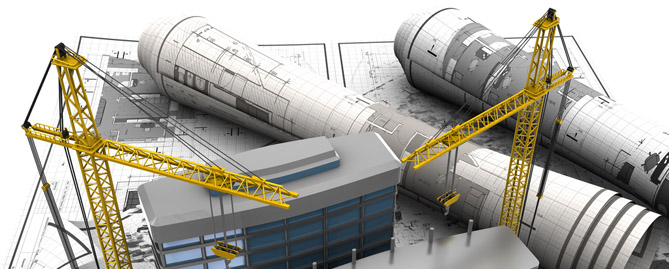
\includegraphics[width=1.15\textwidth]{../Figures/MSc_CE.jpg}
};
\end{tikzpicture}

\end{frame}
\hoffset=0in

%%%%%%%%%%%%%%%%%%%%%%%%%%%%%%%%%%%%%%

%\hoffset=-.8in
\begin{frame}[plain, fragile]

\frametitle{Scope: Program Families}

% if time add another program family example

\begin{tikzpicture}[remember picture,overlay]
\node [xshift=0cm,yshift=-3.cm] at (current page.center)
{
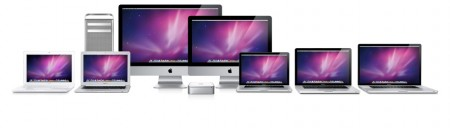
\includegraphics[width=1.2\textwidth]{../Figures/apple-mac-products-450x128.jpg}
};
\end{tikzpicture}

\begin{tikzpicture}[remember picture,overlay]
\node [xshift=0cm,yshift=1.cm] at (current page.center)
{
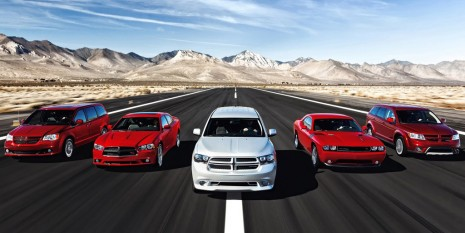
\includegraphics[width=0.8\textwidth]{../Figures/dodge-lineup.jpg}
};
\end{tikzpicture}

\end{frame}
\hoffset=0in

%%%%%%%%%%%%%%%%%%%%%%%%%%%%%%%%%%%%%%

%\hoffset=-.8in
\begin{frame}[plain, fragile]

\frametitle{Scope: End User Developers} 
% end user developers solving physics problems

\begin{tikzpicture}[remember picture,overlay]
\node [xshift=0cm,yshift=-0.2cm] at (current page.center)
{
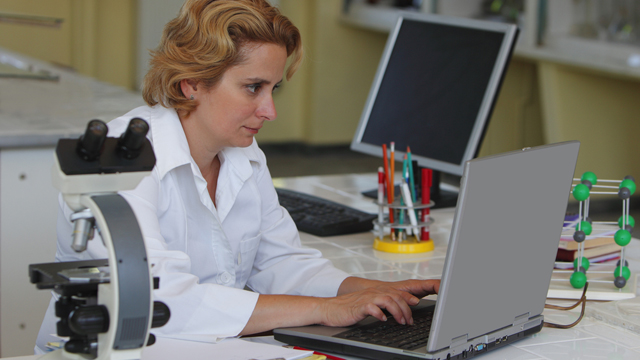
\includegraphics[width=1\textwidth]{../Figures/ScientistAtAComputer.jpg}
};
\end{tikzpicture}

\end{frame}
\hoffset=0in

%%%%%%%%%%%%%%%%%%%%%%%%%%%%%%%%%%%%%%

%\hoffset=-.8in
\begin{frame}[plain, fragile]

\frametitle{Scope: Physical Science} %replace with pictures

\begin{tikzpicture}[remember picture,overlay]
\node [xshift=3.75cm,yshift=0.9cm] at (current page.center)
{
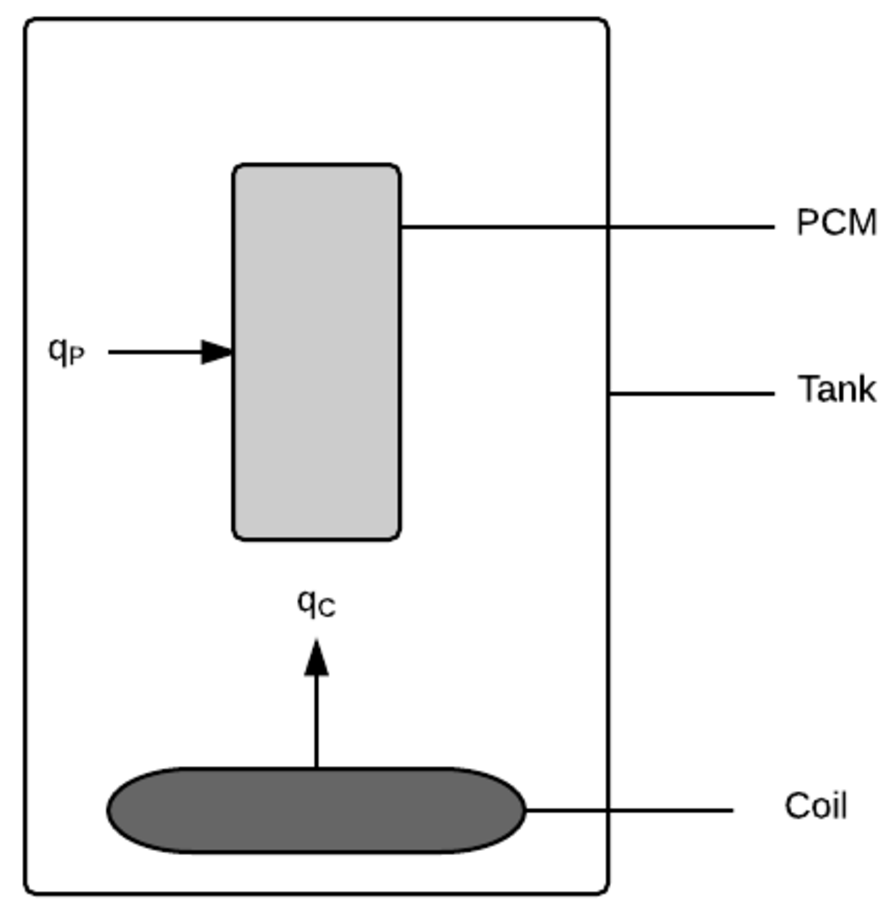
\includegraphics[width=0.4\textwidth]{../Figures/Tank.pdf}
};
\end{tikzpicture}

\begin{tikzpicture}[remember picture,overlay]
\node [xshift=-3.5cm,yshift=1.55cm] at (current page.center)
{
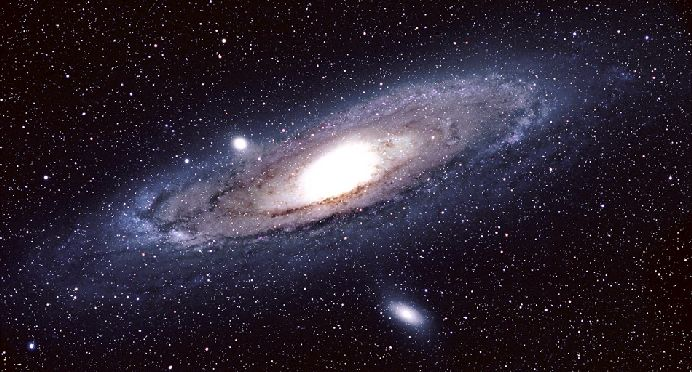
\includegraphics[width=0.5\textwidth]{../Figures/m31_jg.jpg}
};
\end{tikzpicture}

\begin{tikzpicture}[remember picture,overlay]
\node [xshift=0.1cm,yshift=0.8cm] at (current page.center)
{
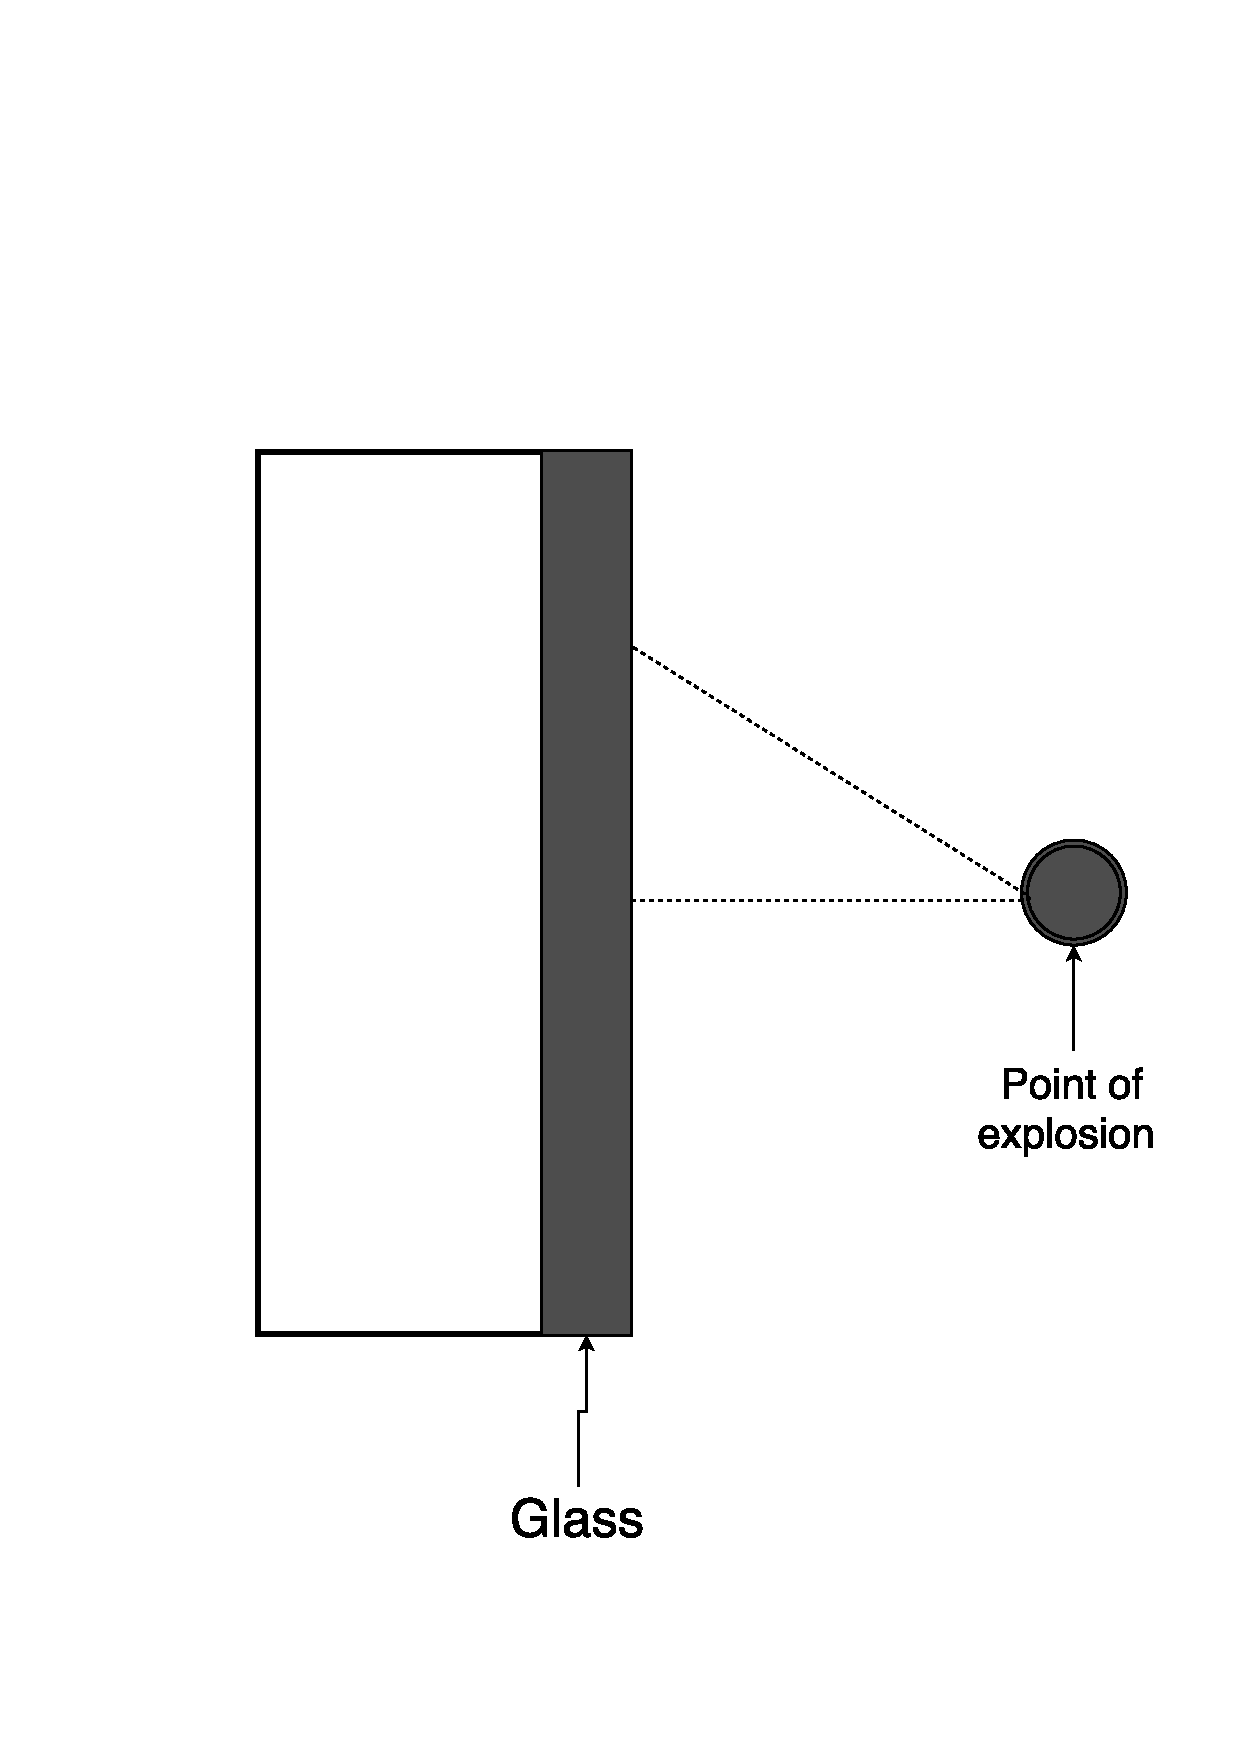
\includegraphics[width=0.3\textwidth]{../Figures/physicalsystimage.pdf}
};
\end{tikzpicture}

\begin{tikzpicture}[remember picture,overlay]
\node [xshift=-3.5cm,yshift=-2.25cm] at (current page.center)
{
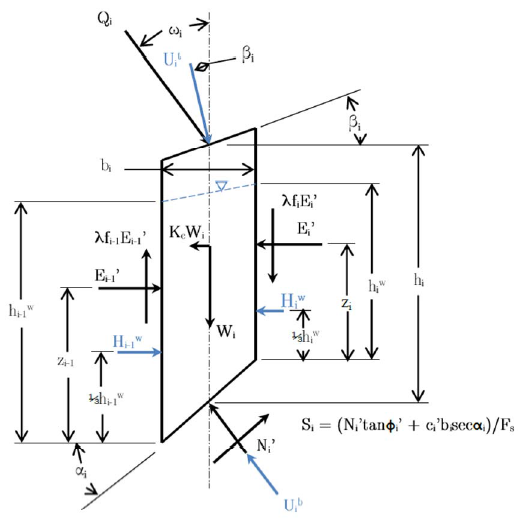
\includegraphics[width=0.4\textwidth]{../Figures/ForceDiagram.png}
};
\end{tikzpicture}

\begin{tikzpicture}[remember picture,overlay]
\node [xshift=0.5cm,yshift=-2.75cm] at (current page.center)
{
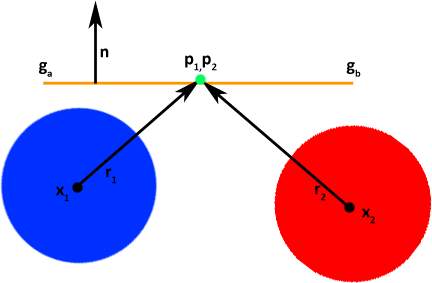
\includegraphics[width=0.3\textwidth]{../Figures/grooveJoint.png}
};
\end{tikzpicture}

\begin{tikzpicture}[remember picture,overlay]
\node [xshift=4.25cm,yshift=-2.75cm] at (current page.center)
{
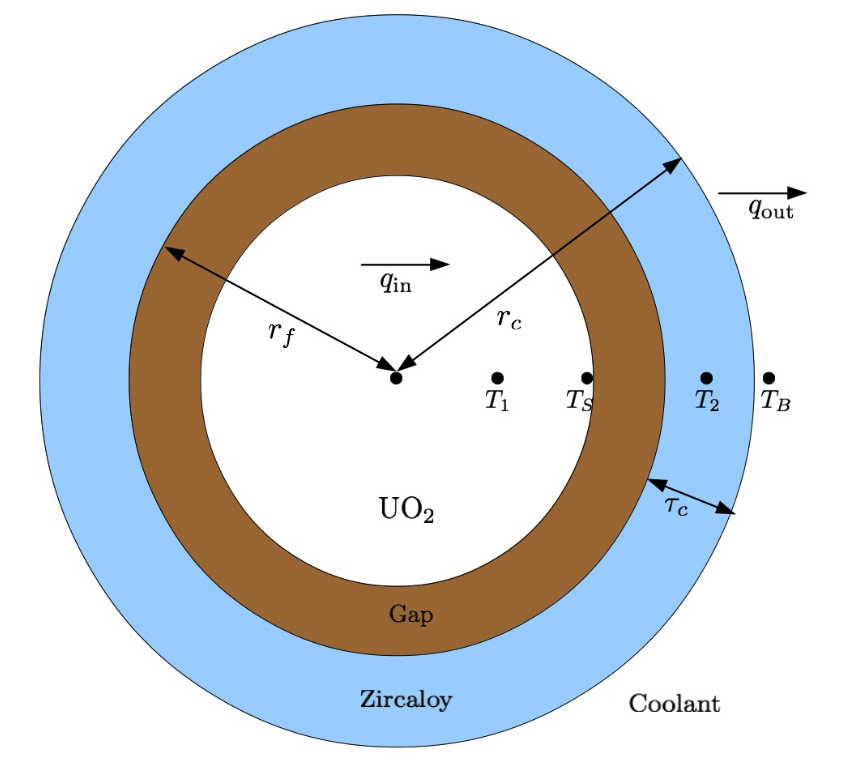
\includegraphics[width=0.3\textwidth]{../Figures/fuelpin.png}
};
\end{tikzpicture}

\end{frame}
\hoffset=0in

%%%%%%%%%%%%%%%%%%%%%%%%%%%%%%%%%%%%%%

%\section[Motivation]{Motivation}

%%%%%%%%%%%%%%%%%%%%%%%%%%%%%%%%%%%%%%

%\hoffset=-.8in
\begin{frame}[plain, fragile]

\frametitle{Motivation: Safety}

% picture of reactor, MRI

\begin{tikzpicture}[remember picture,overlay]
\node [xshift=-0.1cm,yshift=0.75cm] at (current page.center)
{
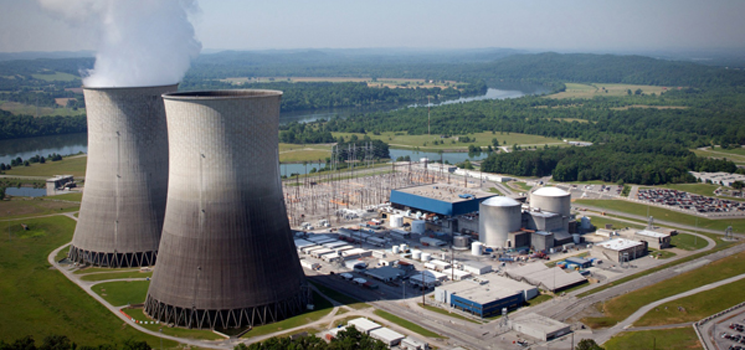
\includegraphics[width=1.1\textwidth]{../Figures/nuclear_reactor_technologies_home.png}
};
\end{tikzpicture}

\begin{tikzpicture}[remember picture,overlay]
\node [xshift=1.75cm,yshift=-1.75cm] at (current page.center)
{
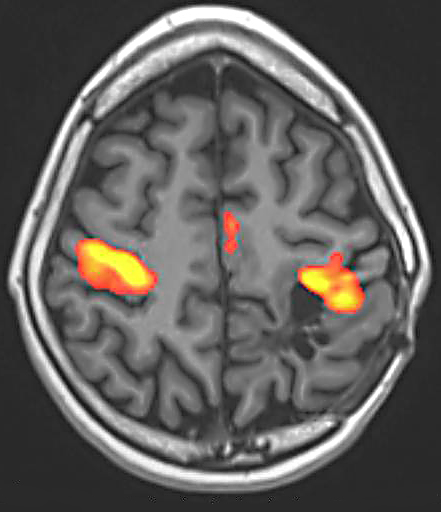
\includegraphics[width=0.4\textwidth]{../Figures/fmri-image.jpg}
};
\end{tikzpicture}

\end{frame}
\hoffset=0in

%%%%%%%%%%%%%%%%%%%%%%%%%%%%%%%%%%%%%%

%\hoffset=-.8in
\begin{frame}[plain, fragile]

\frametitle{Motivation: (Re)certification}

% picture of stamp

\begin{tikzpicture}[remember picture,overlay]
\node [xshift=0cm,yshift=0cm] at (current page.center)
{

\includegraphics[width=0.8\textwidth]{../Figures/certified.jpg}
};
\end{tikzpicture}

\end{frame}
\hoffset=0in

%%%%%%%%%%%%%%%%%%%%%%%%%%%%%%%%%%%%%%

\begin{frame}

\frametitle{Motivation: Improve Quality}

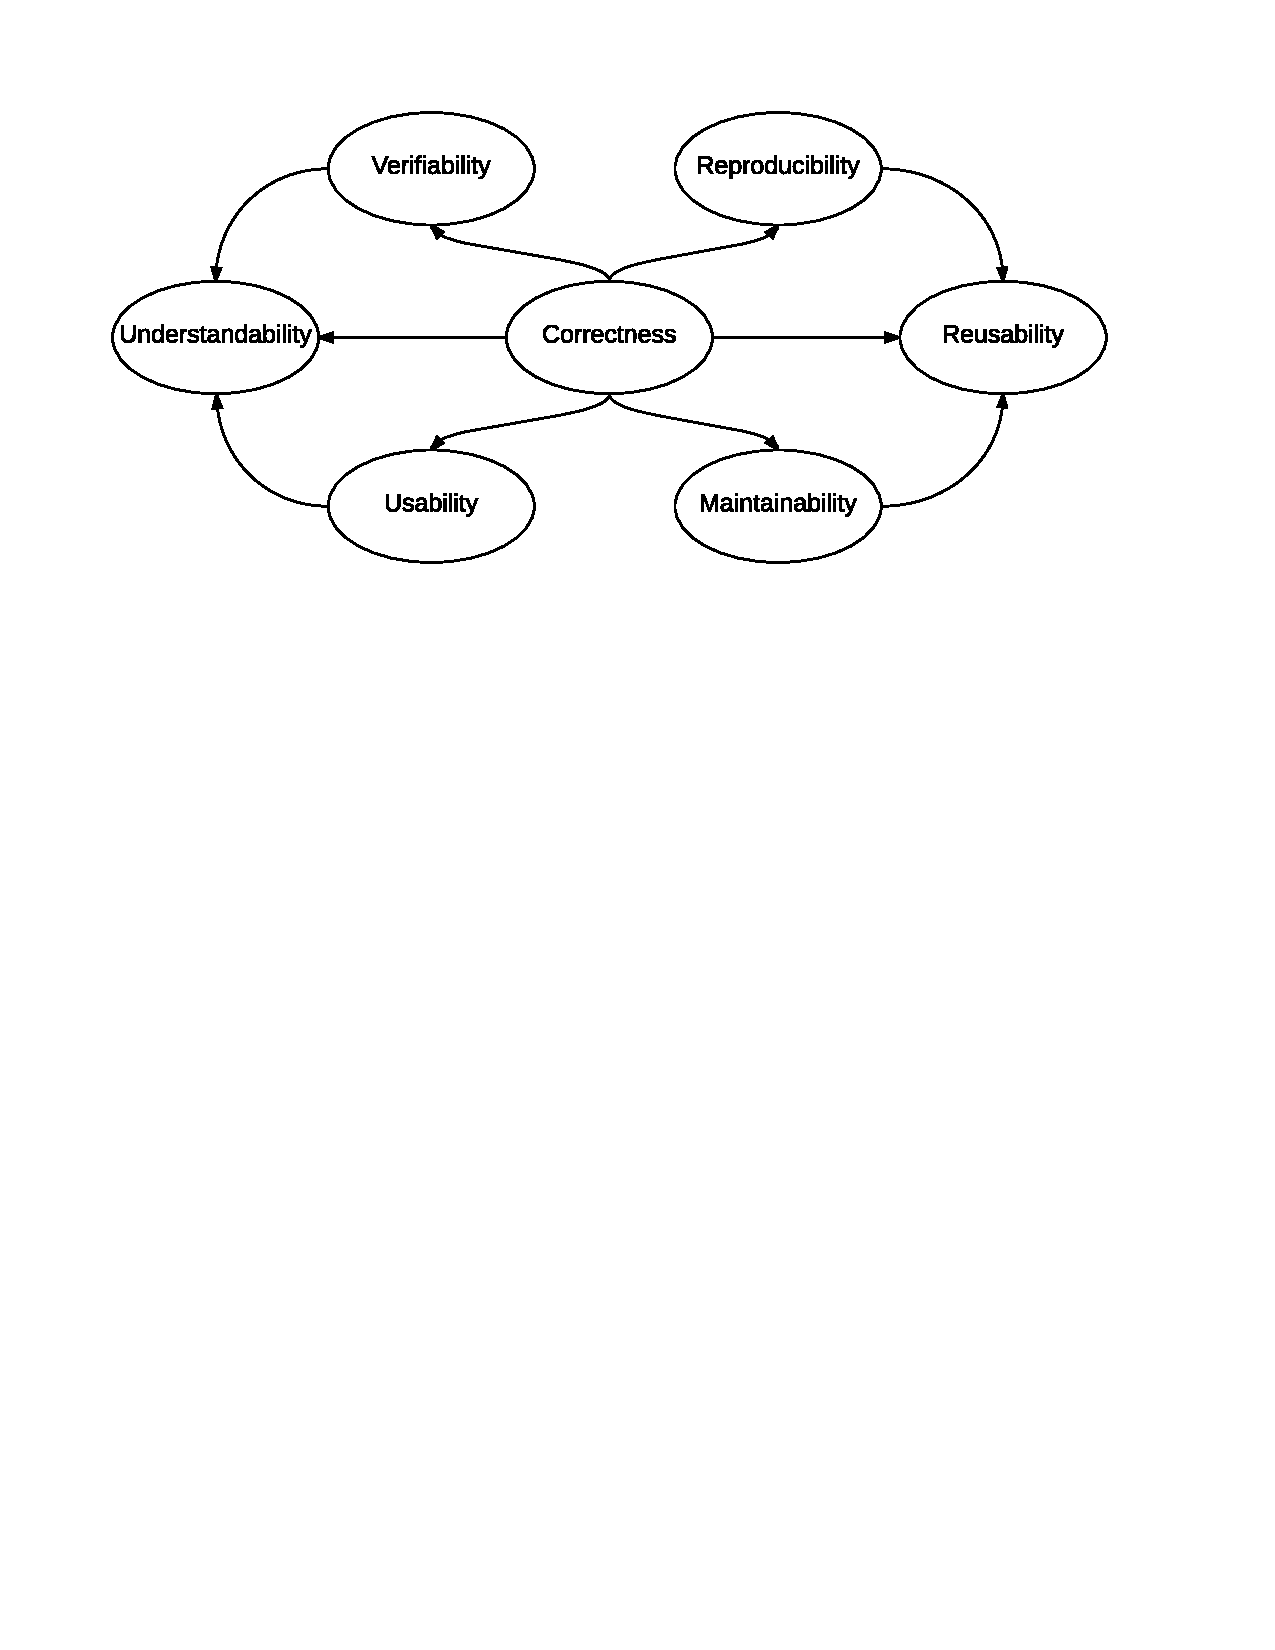
\includegraphics[width=1.\textwidth]{../Figures/RelationBWQualities.pdf}

\end{frame}

%%%%%%%%%%%%%%%%%%%%%%%%%%%%%%%%%%%%%%

% \section[Curr.\ Approach]{Current Approach to Developing SCS}

% %%%%%%%%%%%%%%%%%%%%%%%%%%%%%%%%%%%%%%

% \begin{frame}

% \frametitle{Current Approach}

% \begin{itemize}
% \item Agile like \citep{CarverEtAl2007}
% \item Amethododical \citep{Kelly2013}
% \item Knowledge acquisition driven \citep{Kelly2015}
% \item Each stage reports counterproductive \citep{Roache1998}
% \item Limited tool use \citep{Wilson2006}
% \item Limited testing of code \citep{KellyAndSanders2008a}
% \item Lack of understanding of testing \citep{Merali2010}
% \item Missed opportunities for reuse \citep{Owen1998} 
%  %-- 37 of 52 triangular mesh generators
%  % implemented the same triangulation algorithm
% \item Emphasis on:
% \begin{enumerate}
% \item Science~\citep{Kelly2007}
% \item Code
% \end{enumerate}
% \end{itemize}

% \end{frame}

% %%%%%%%%%%%%%%%%%%%%%%%%%%%%%%%%%%%%%%

% \begin{frame}

% \frametitle{Challenges for DDD}

% \begin{itemize}
% \item Up front requirements
% \item Rapid change for numerical algorithms
% \item Information duplication
% \item Synchronization headaches between artifacts
% \item Perceived over-emphasis on non-executable artifacts
% %Parnas paper - people do not like docs, vicious cycle
% \end{itemize}

% \end{frame}

%%%%%%%%%%%%%%%%%%%%%%%%%%%%%%%%%%%%%%

%\section[DDD]{Document Driven Design}

%%%%%%%%%%%%%%%%%%%%%%%%%%%%%%%%%%%%%%

\begin{frame}

\frametitle{Current Approach}

\begin{itemize}
\item Agile like \cite{CarverEtAl2007}
\item Amethododical \cite{Kelly2013}
\item Knowledge acquisition driven \cite{Kelly2015}
\item Each stage reports counterproductive \cite{Roache1998}
\item Limited tool use \cite{Wilson2006}
\item Limited testing of code \cite{KellyAndSanders2008a}
\item Lack of understanding of testing \cite{Merali2010}
\item Missed opportunities for reuse \cite{Owen1998} 
 %-- 37 of 52 triangular mesh generators
 % implemented the same triangulation algorithm
\item Emphasis on:
\begin{enumerate}
\item Science~\cite{Kelly2007}
\item Code
\end{enumerate}
\end{itemize}

\end{frame}

%%%%%%%%%%%%%%%%%%%%%%%%%%%%%%%%%%%%%%

\begin{frame}

\frametitle{Documentation Advantages}

\begin{itemize}
\item Improves verifiability, reusability, reproducibility, etc.
\item From \cite{Parnas2010}
\begin{itemize}
\item easier reuse of old designs
\item better communication about requirements
\item more useful design reviews
\item easier integration of separately written modules
\item more effective code inspection
\item more effective testing
\item more efficient corrections and improvements
\end{itemize}
\item New doc found 27 errors \cite{SmithAndKoothoor2016}
\item Developers see advantage \cite{SmithJegatheesanAndKelly2016}
\end{itemize}

\end{frame}

%%%%%%%%%%%%%%%%%%%%%%%%%%%%%%%%%%%%%%

\begin{frame}

\frametitle{Study Of Documentation in SC \cite{SmithJegatheesanAndKelly2016}}

\begin{enumerate}

\item Select 5 small to medium size SCS
\item Interview code owners
\item Redevelop using Document Driven Design (DDD)
\item Interview code owners
\item Analyze responses

\end{enumerate}

\end{frame}

%%%%%%%%%%%%%%%%%%%%%%%%%%%%%%%%%%%%%%

%\hoffset=-.6in %removing side bar for these frames

\begin{frame}

\frametitle{Summary of Case Studies}

  \begin{tabular}{lrlclccccc}
    \toprule
    & \textbf{LOC} & \textbf{Lng} & \textbf{ND} & \textbf{Ag} 
    & \textbf{SE} & \textbf{Prg} & \textbf{Tst} & \textbf{VC} & \textbf{Bug}\\

    \midrule \textbf{SWHS} & 1000 & F77 & 1 & 5 & \cross &
                                                           \checkmark
                                 & \cross & \cross & \cross \\
	  
    \textbf{Astro} &5000 & C & 2 & 10 & \ding{55} &
                                                             \checkmark & \cross & \cross & \cross \\
      
    \textbf{Glass} & 1300 & F90 & 1 & $<$1 & \cross &
                                                               \checkmark & \cross & \cross & \cross \\

    \textbf{Soil} & 800 &  M & 1 & 5 & \checkmark &
                                                             \checkmark & \checkmark & \checkmark & \cross \\
	  
    \textbf{Neuro} & 1000 & M & 1 & 5 & \checkmark &
                                                              \checkmark & \cross & \checkmark & \cross \\
	  
    \textbf{Acoust} & 200 & M & 4 & 2.5 & \cross &
                                                            \checkmark & \cross & \cross & \cross \\
	  		
    \bottomrule
				
  \end{tabular}  

\end{frame}
%\hoffset=0in %resetting side bar

%%%%%%%%%%%%%%%%%%%%%%%%%%%%%%%%%%%%%%

\begin{frame}

\frametitle{Perceived Advantages from Participants}

\begin{itemize}
\item \structure{Documentation of assumptions}
\item \structure{All variables have explicit units}
\item SRS helpful with new graduate students
\item Modules result in more user friendly code
\item \structure{Traceability between modules and requirements useful}
\item Better organized code
\item Information sharing on design choices
\item \structure{Detailed record of knowledge capital}
\item Code is produced to make testing easier
\end{itemize}

\end{frame}

%%%%%%%%%%%%%%%%%%%%%%%%%%%%%%%%%%%%%%

%\subsection[Disadvantages]{Disadvantages}

%%%%%%%%%%%%%%%%%%%%%%%%%%%%%%%%%%%%%%

\begin{frame}

\frametitle{Disadvantages (Perceived and Real)}

\begin{itemize}
\item SRS is too long
\item SRS is not necessary
\item DDD will not work in reality, since needs upfront requirements
\item Too much SE jargon
\item Difficult without a team of people
\item Too difficult to maintain
\item Not amenable to change
\item Too tied to waterfall process
\item Reports counterproductive \cite{Roache1998}
\end{itemize}

\textbf{The Solution?}

\end{frame}

%%%%%%%%%%%%%%%%%%%%%%%%%%%%%%%%%%%%%%

%\section[Drasil]{Drasil}

%%%%%%%%%%%%%%%%%%%%%%%%%%%%%%%%%%%%%%

%\subsection[Overview]{Overview of Drasil}

%%%%%%%%%%%%%%%%%%%%%%%%%%%%%%%%%%%%%%

\begin{frame}

\includegraphics[width=1\textwidth]{../Figures/generate_all_the_things.jpg}
\end{frame}

%%%%%%%%%%%%%%%%%%%%%%%%%%%%%%%%%%%%%%

\begin{frame}

\frametitle{Knowledge Capture}

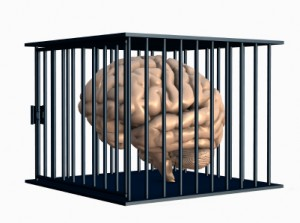
\includegraphics[width=1.0\textwidth]{../Figures/KC.jpg}

\end{frame}

%%%%%%%%%%%%%%%%%%%%%%%%%%%%%%%%%%%%%%

\begin{frame}

\frametitle{Drasil}
\vspace{-1cm}
\begin{center}
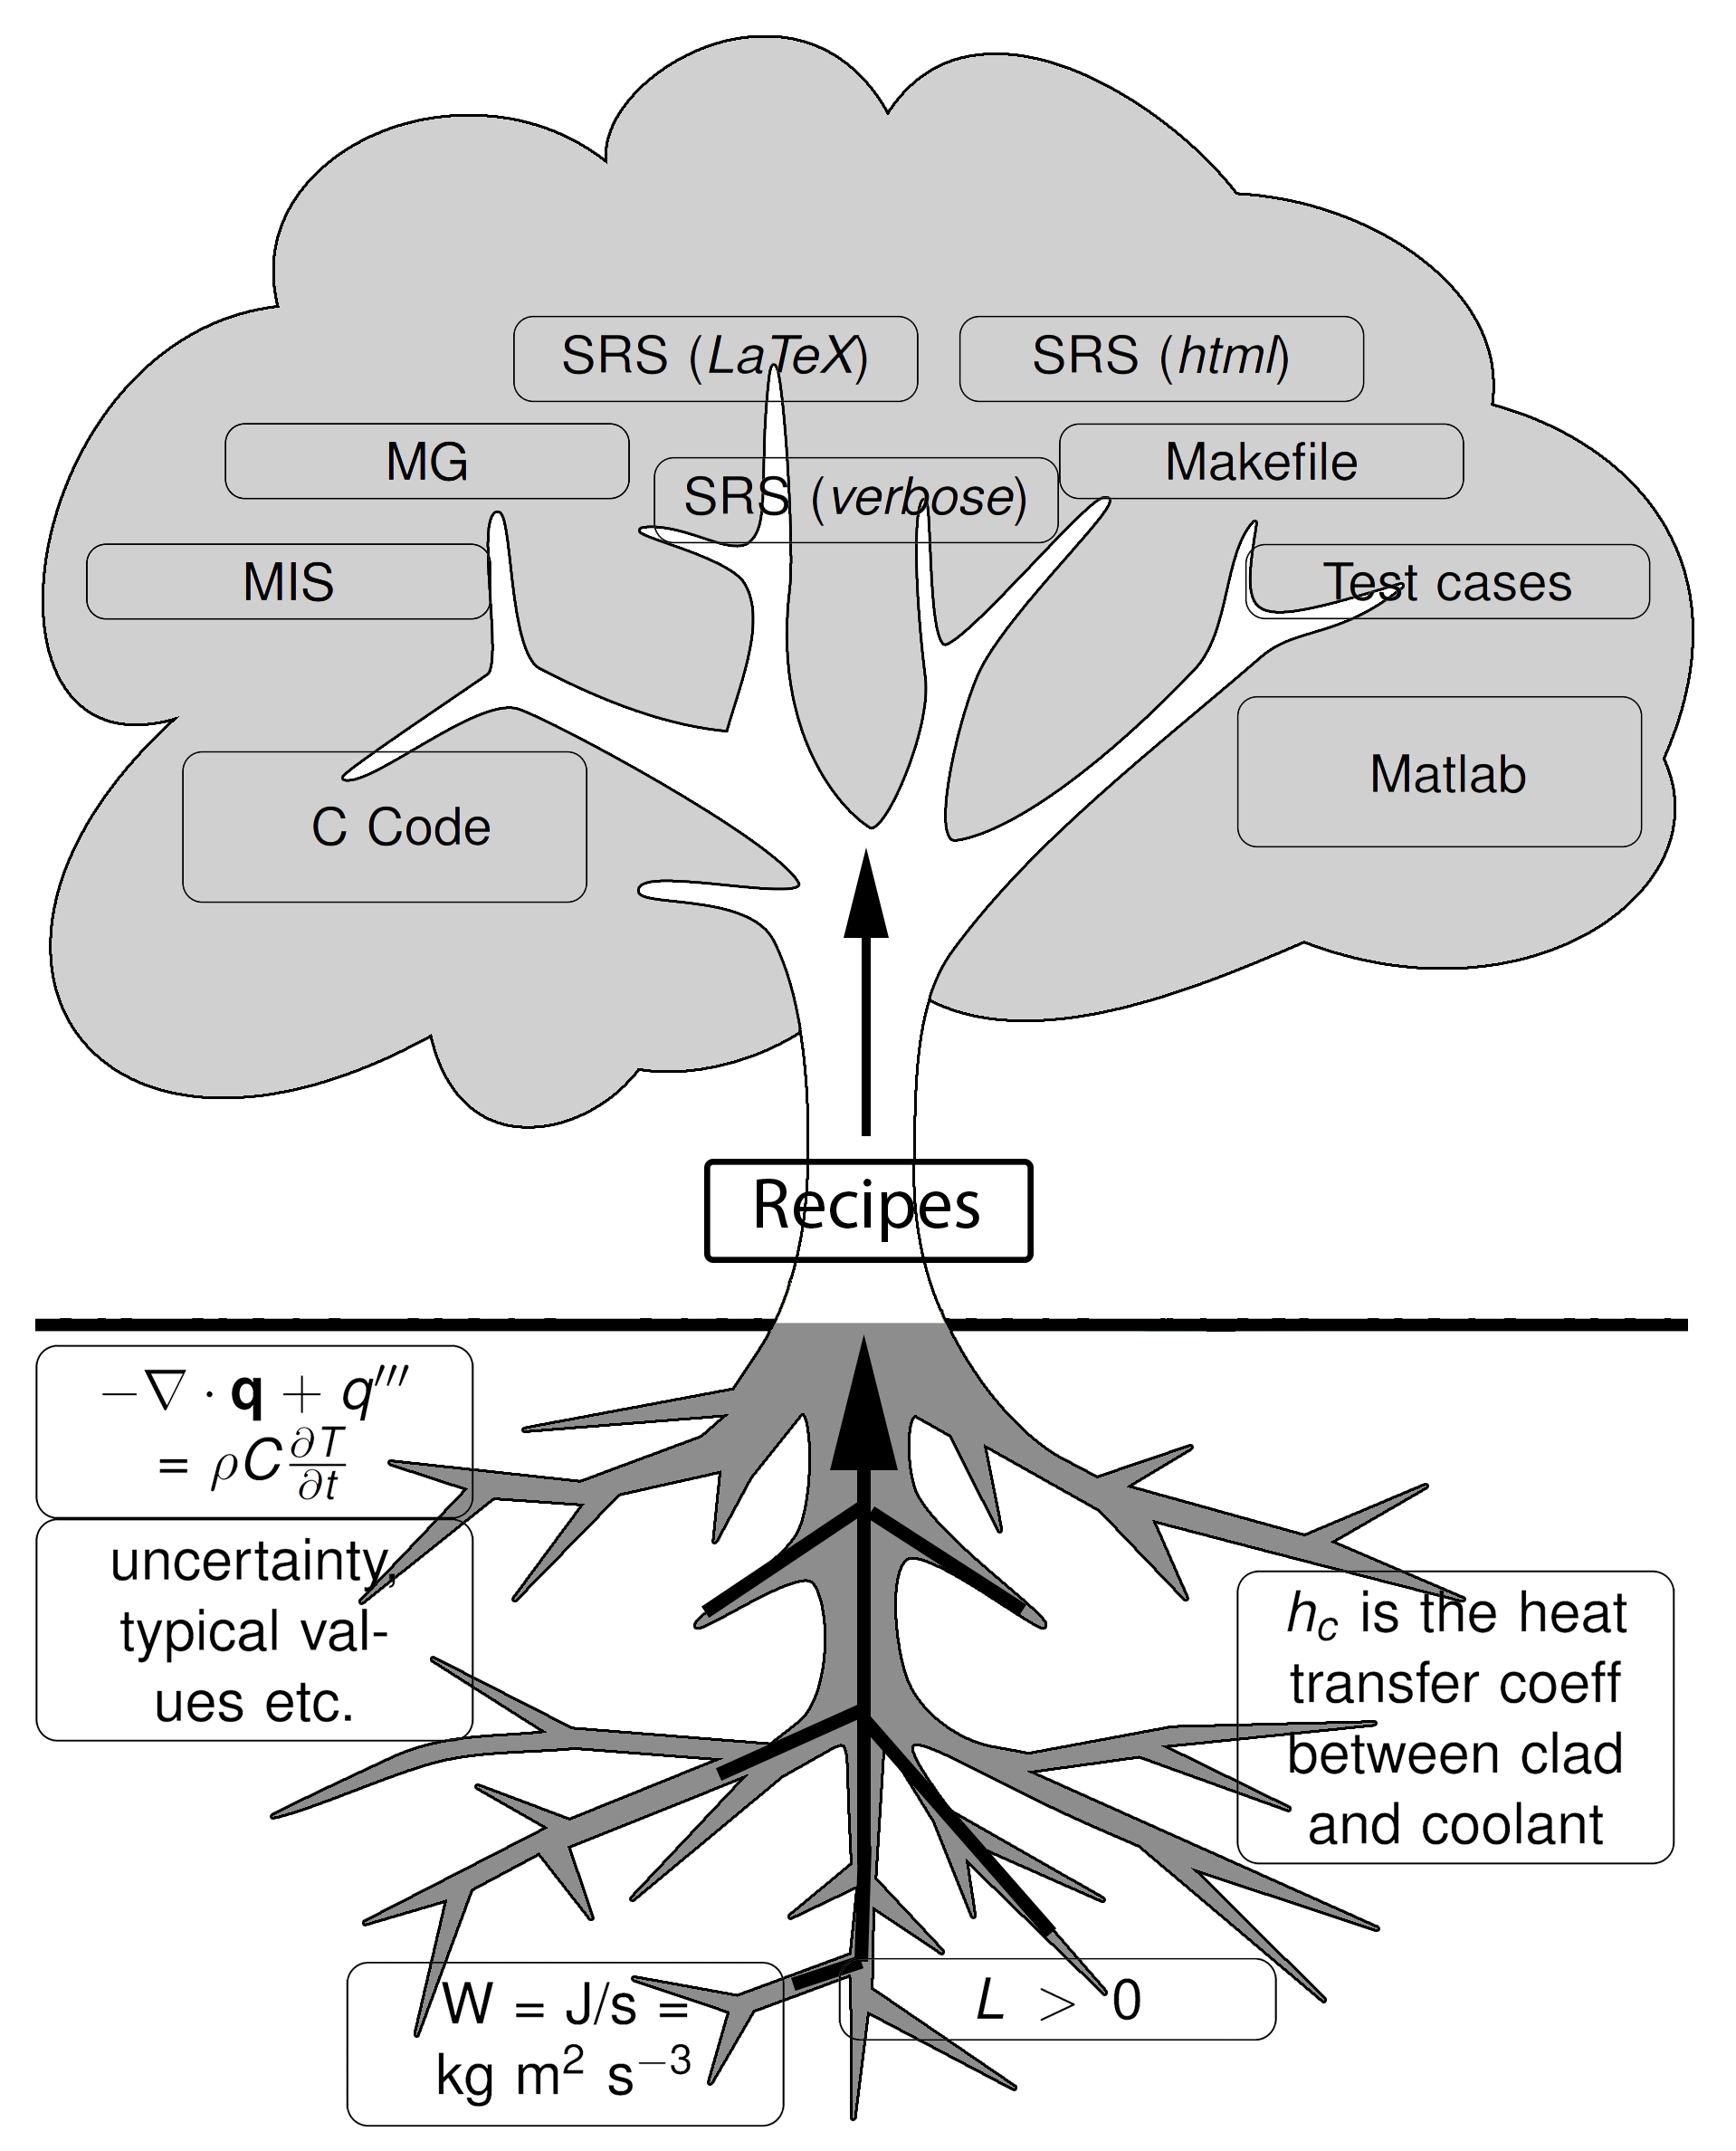
\includegraphics[height=20em]{../Figures/tree.png}
\end{center}
\end{frame}

%%%%%%%%%%%%%%%%%%%%%%%%%%%%%%%%%%%%%

\begin{frame}
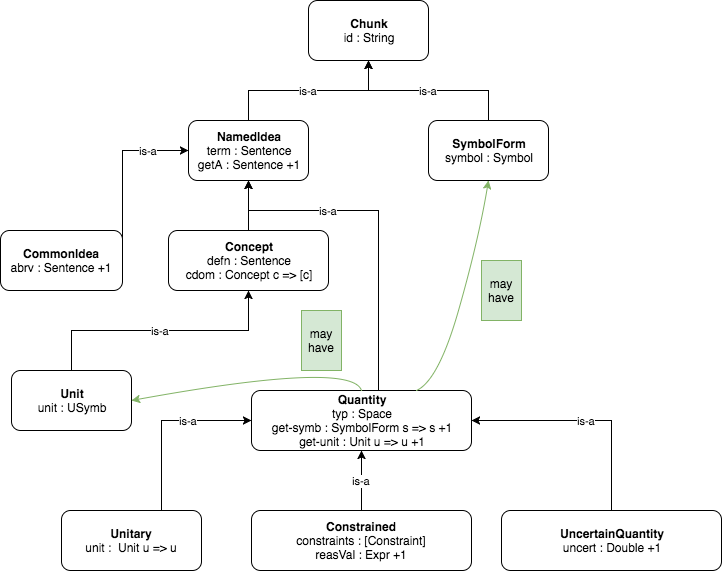
\includegraphics[width=1\textwidth]{../Figures/class_hierarchy.png}
\end{frame}

%%%%%%%%%%%%%%%%%%%%%%%%%%%%%%%%%%%%%

% \begin{frame}

% \frametitle{Knowledge Based Approach}

% \begin{itemize}
% \item Capture knowledge
% \item From one ``source'' recipes to generate artifacts
% \item Automated
% \item Inspired by Knuth's Literate Programming
% \end{itemize}
% \end{frame}

%%%%%%%%%%%%%%%%%%%%%%%%%%%%%%%%%%%%%%

%\subsection[Example]{Example}

%%%%%%%%%%%%%%%%%%%%%%%%%%%%%%%%%%%%%%

\begin{frame}

\frametitle{$J_{\mbox{tol}}$ in SRS.pdf}
\begin{center}
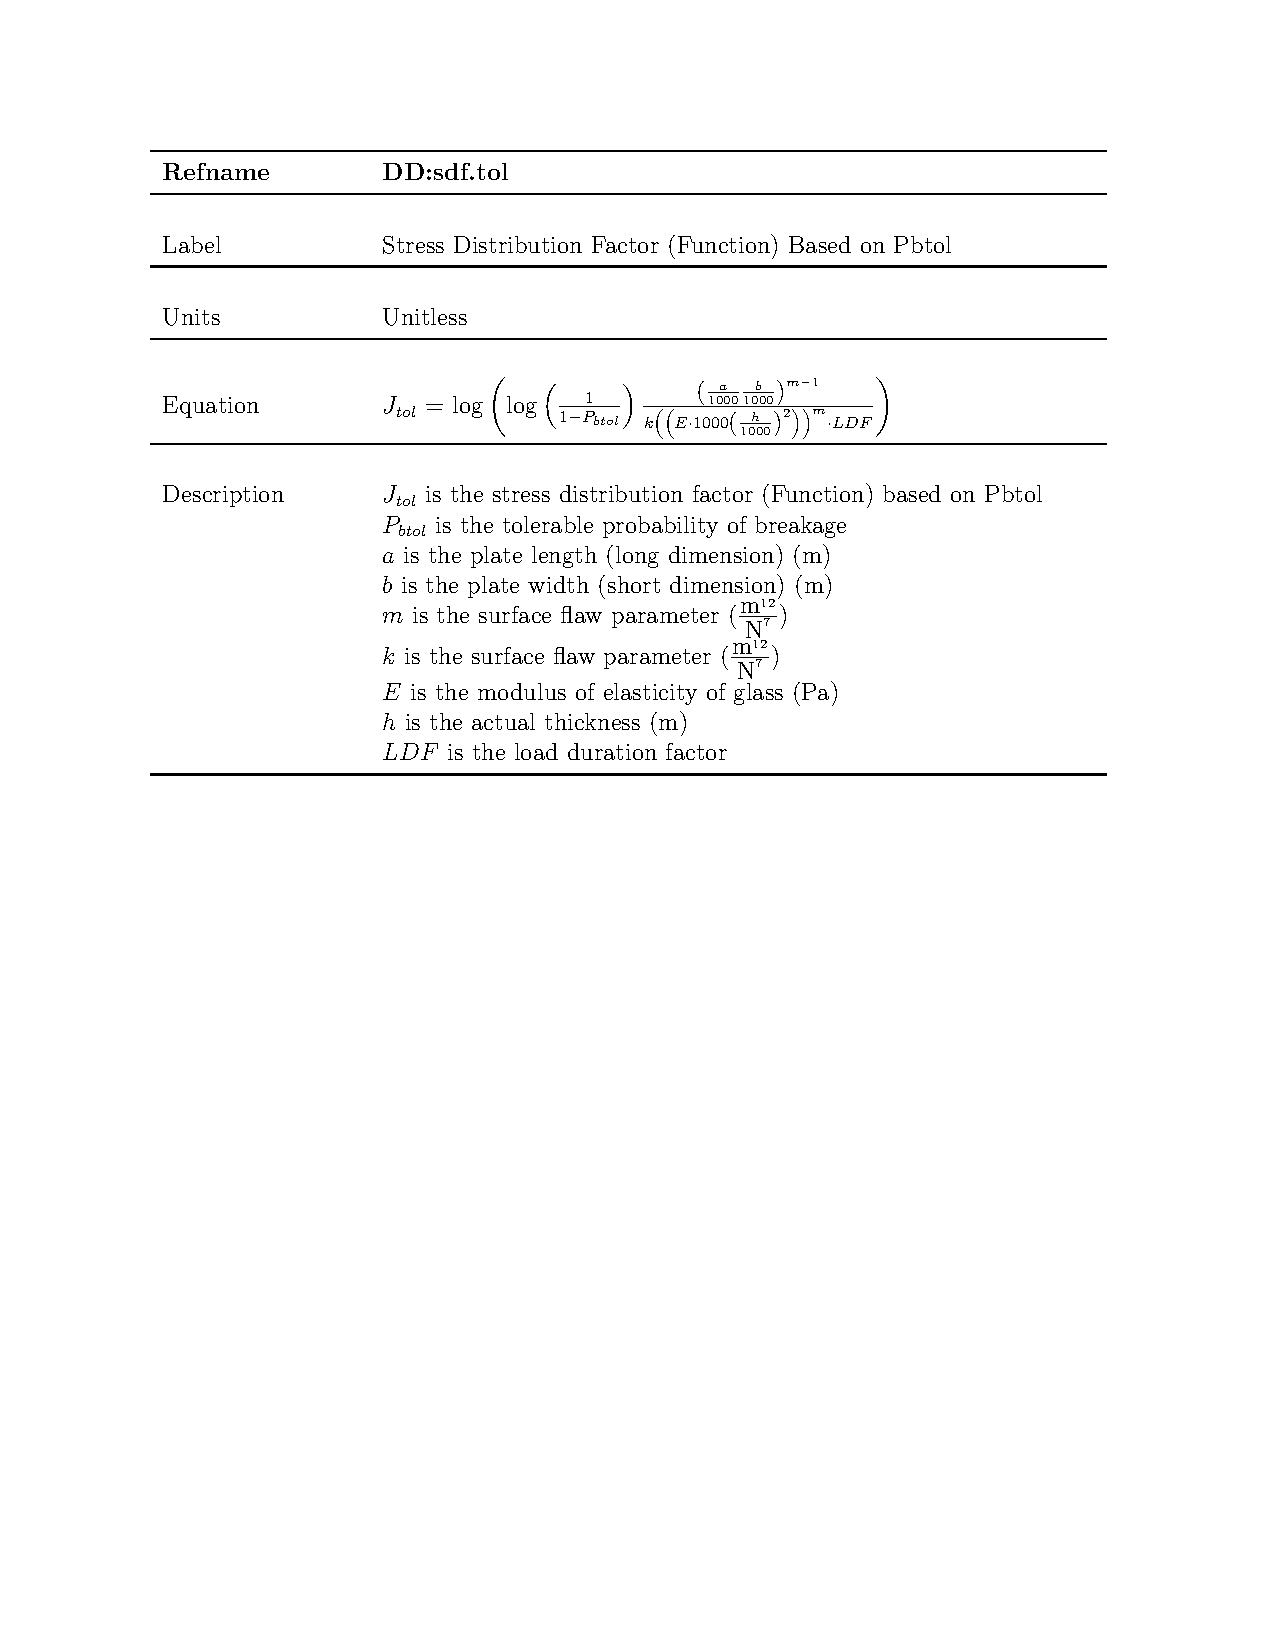
\includegraphics[width=1.0\textwidth]{../Figures/Jtol_pdf.pdf}
\end{center}
\end{frame}

%%%%%%%%%%%%%%%%%%%%%%%%%%%%%%%%%%%%%

\begin{frame}[plain, fragile]

\frametitle{$J_{\mbox{tol}}$ in SRS.tex}
~\\
\begin{lstlisting}
\noindent \begin{minipage}{\textwidth}
\begin{tabular}{p{0.2\textwidth} p{0.73\textwidth}}
\toprule \textbf{Refname} & \textbf{DD:sdf.tol}
\phantomsection 
\label{DD:sdf.tol}
\\ \midrule \\
Label & $J_{tol}$
\\ \midrule \\
Units & 
\\ \midrule \\
Equation & $J_{tol}$ =
           $\log\left(\log\left(\frac{1}{1-P_{btol}}\right)\frac{\left(\frac{a}{1000}\frac{b}{1000}\right)^{m-1}}{k\left(\left(E*1000\right)\left(\frac{h}{1000}\right)^{2}\right)^{m}*LDF}\right)$
\\ \midrule \\
Description & $J_{tol}$ is the stress distribution factor (Function) based on
              Pbtol\newline$P_{btol}$ is the tolerable probability of breakage ...
\end{minipage}\\
\end{lstlisting}
\end{frame}

%%%%%%%%%%%%%%%%%%%%%%%%%%%%%%%%%%%%%%

\begin{frame}[plain, fragile]

\frametitle{$J_{\mbox{tol}}$ in SRS.html}

\begin{lstlisting}

<a id="">
<div class="equation">
<em>J<sub>tol</sub></em> = log(log(<div class="fraction">
<span class="fup">
1
</span>
<span class="fdn">
1 &minus; <em>P<sub>btol</sub></em>
</span>
</div>)<div class="fraction">
<span class="fup">
(<div class="fraction">
<span class="fup">
<em>a</em>
</span>
<span class="fdn">
1000
</span>
</div><div class="fraction">
...
\end{lstlisting}

\end{frame}
%%%%%%%%%%%%%%%%%%%%%%%%%%%%%%%%%%%%%

\begin{frame}[plain, fragile]

\frametitle{$J_{\mbox{tol}}$ in Python}

\begin{lstlisting}
def calc_j_tol(inparams):
    j_tol = math.log((math.log(1.0 / (1.0 - inparams.pbtol))) * ((((inparams.a / 1000.0) * (inparams.b / 1000.0)) ** (inparams.m - 1.0)) / ((inparams.k * (((inparams.E * 1000.0) * ((inparams.h / 1000.0) ** 2.0)) ** inparams.m)) * inparams.ldf)))
    return j_tol
\end{lstlisting}
\end{frame}

%%%%%%%%%%%%%%%%%%%%%%%%%%%%%%%%%%%%%%

\begin{frame}[plain, fragile]

\frametitle{$J_{\mbox{tol}}$ in Java}

\begin{lstlisting}
public static double calc_j_tol(InputParameters inparams) {
        double j_tol = Math.log((Math.log(1.0 / (1.0 - inparams.pbtol))) * ((Math.pow((inparams.a / 1000.0) * (inparams.b / 1000.0), inparams.m - 1.0)) / ((inparams.k * (Math.pow((inparams.E * 1000.0) * (Math.pow(inparams.h / 1000.0, 2.0)), inparams.m))) * inparams.ldf)));
        return j_tol;
    }
\end{lstlisting}
\end{frame}

%%%%%%%%%%%%%%%%%%%%%%%%%%%%%%%%%%%%%%

\begin{frame}[plain, fragile]

\frametitle{$J_{\mbox{tol}}$ in Drasil (Haskell)}

\begin{lstlisting}
stressDistFac = makeVC "stressDistFac" (nounPhraseSP 
  $ "stress distribution" ++ " factor (Function)") cJ
sdf_tol = makeVC "sdf_tol" (nounPhraseSP $ 
  "stress distribution" ++
  " factor (Function) based on Pbtol") 
  (sub (eqSymb stressDistFac) (Atomic "tol"))

tolStrDisFac_eq :: Expr
tolStrDisFac_eq = log (log ((1)/((1) - (C pb_tol)))
  * ((Grouping (((C plate_len) / (1000)) * ((C
      plate_width) / (1000))) :^
  ((C sflawParamM) - (1)) / ((C sflawParamK) *
  (Grouping (Grouping ((C mod_elas * 1000) *
  (square (Grouping ((C act_thick) / (1000)))))) :^ 
  (C sflawParamM) * (C lDurFac))))))
tolStrDisFac :: QDefinition
tolStrDisFac = mkDataDef' sdf_tol tolStrDisFac_eq 
  (aGrtrThanB +:+ hRef +:+ ldfRef +:+ pbTolUsr)
\end{lstlisting}
\end{frame}

%%%%%%%%%%%%%%%%%%%%%%%%%%%%%%%%%%%%%%

\begin{frame}[plain, fragile]

\frametitle{$J_{\mbox{tol}}$ without Unit Conversion}

\begin{lstlisting}
tolStrDisFac_eq :: Expr
tolStrDisFac_eq = log (log ((1)/((1) - (C pb_tol)))
  * ((Grouping ((C plate_len) * (C plate_width)) :^
  ((C sflawParamM) - (1)) / ((C sflawParamK) *
  (Grouping (Grouping ((C mod_elas * 1000) *
  (square (Grouping (C act_thick))))) :^ 
  (C sflawParamM) * (C lDurFac))))))
\end{lstlisting}
\end{frame}

%%%%%%%%%%%%%%%%%%%%%%%%%%%%%%%%%%%%%%

%\subsection[SRS]{SRS}

%%%%%%%%%%%%%%%%%%%%%%%%%%%%%%%%%%%%%%

% \hoffset=-.4in %removing side bar for these frames

% \begin{frame}[plain, fragile]

% %\frametitle{SRS for SWHS}

% \begin{center}
% 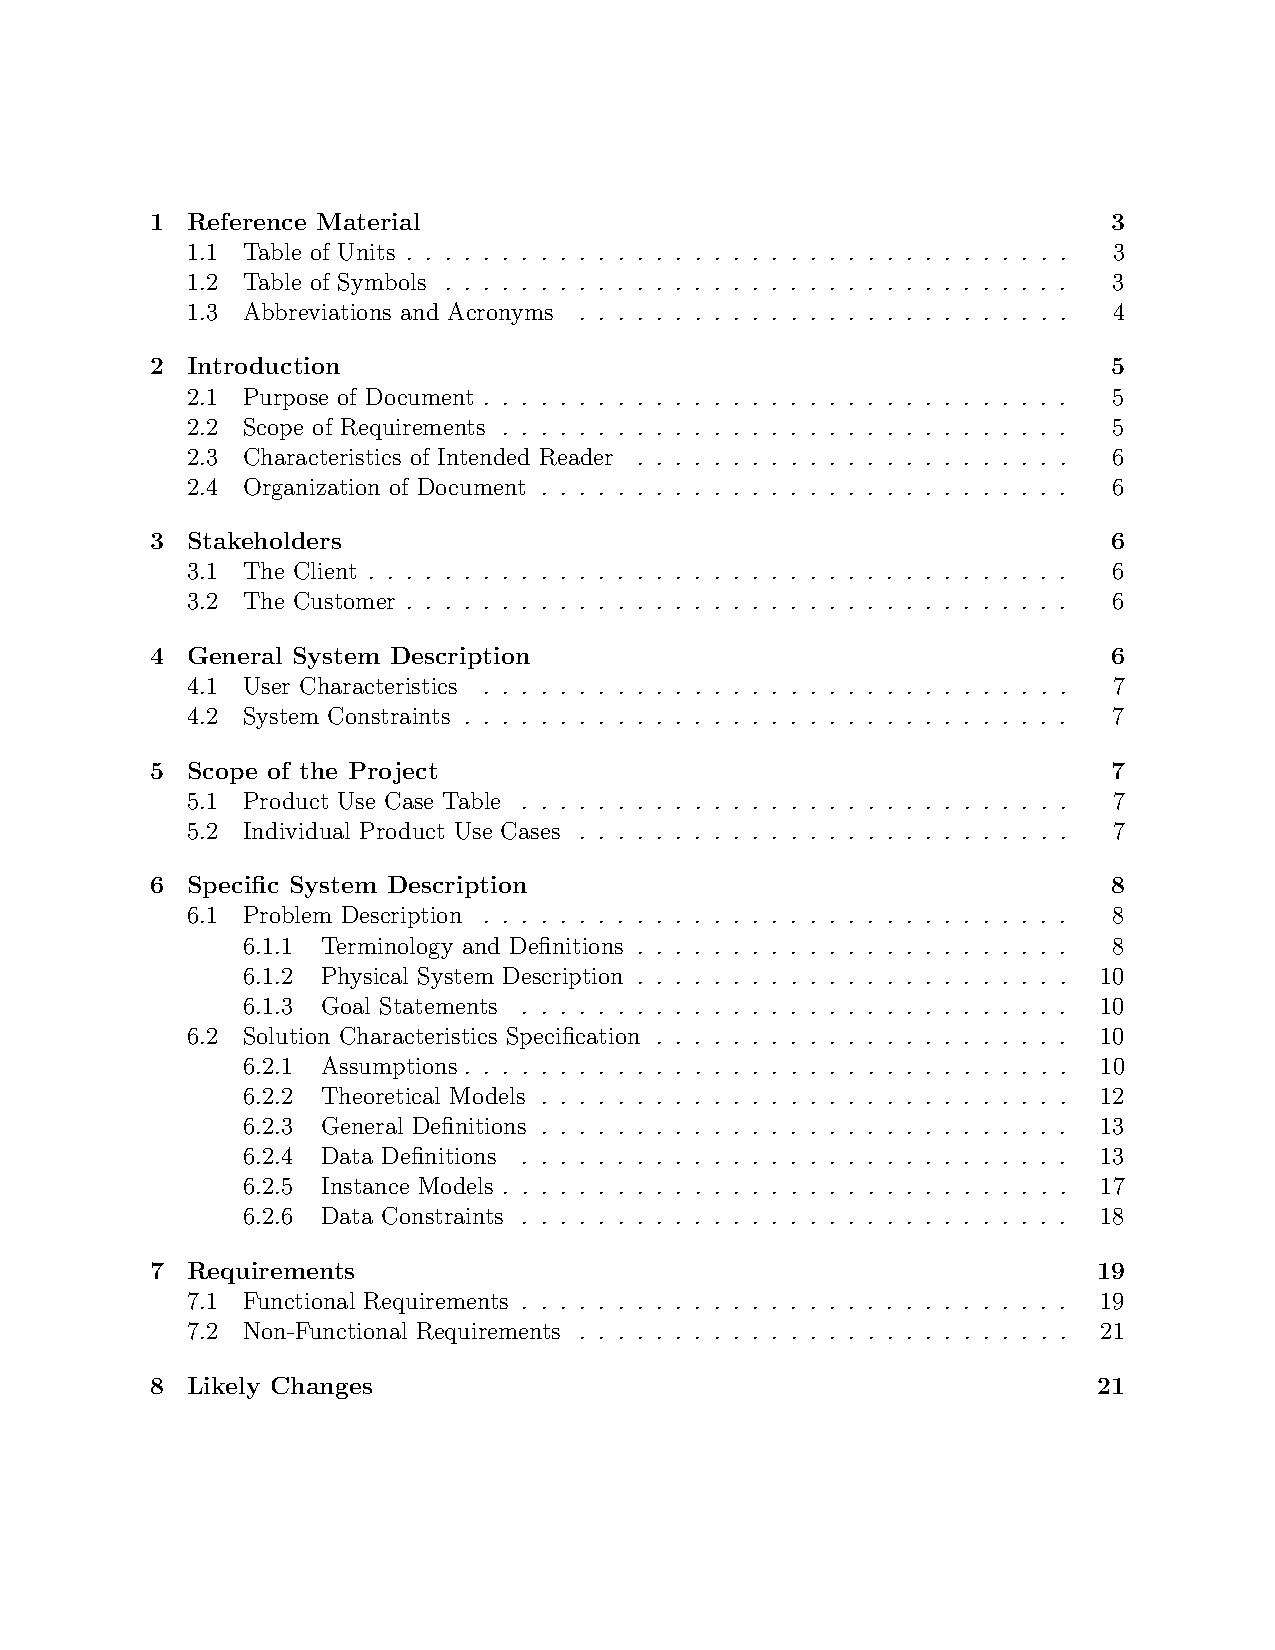
\includegraphics[scale=0.45]{../Figures/TofC.pdf}
% \end{center}

% \end{frame}
% \hoffset=0in

%%%%%%%%%%%%%%%%%%%%%%%%%%%%%%%%%%%%%%

%\hoffset=-.7in %removing side bar for these frames

\begin{frame}[plain, fragile]

\frametitle{Traceability Graph}

\begin{center}
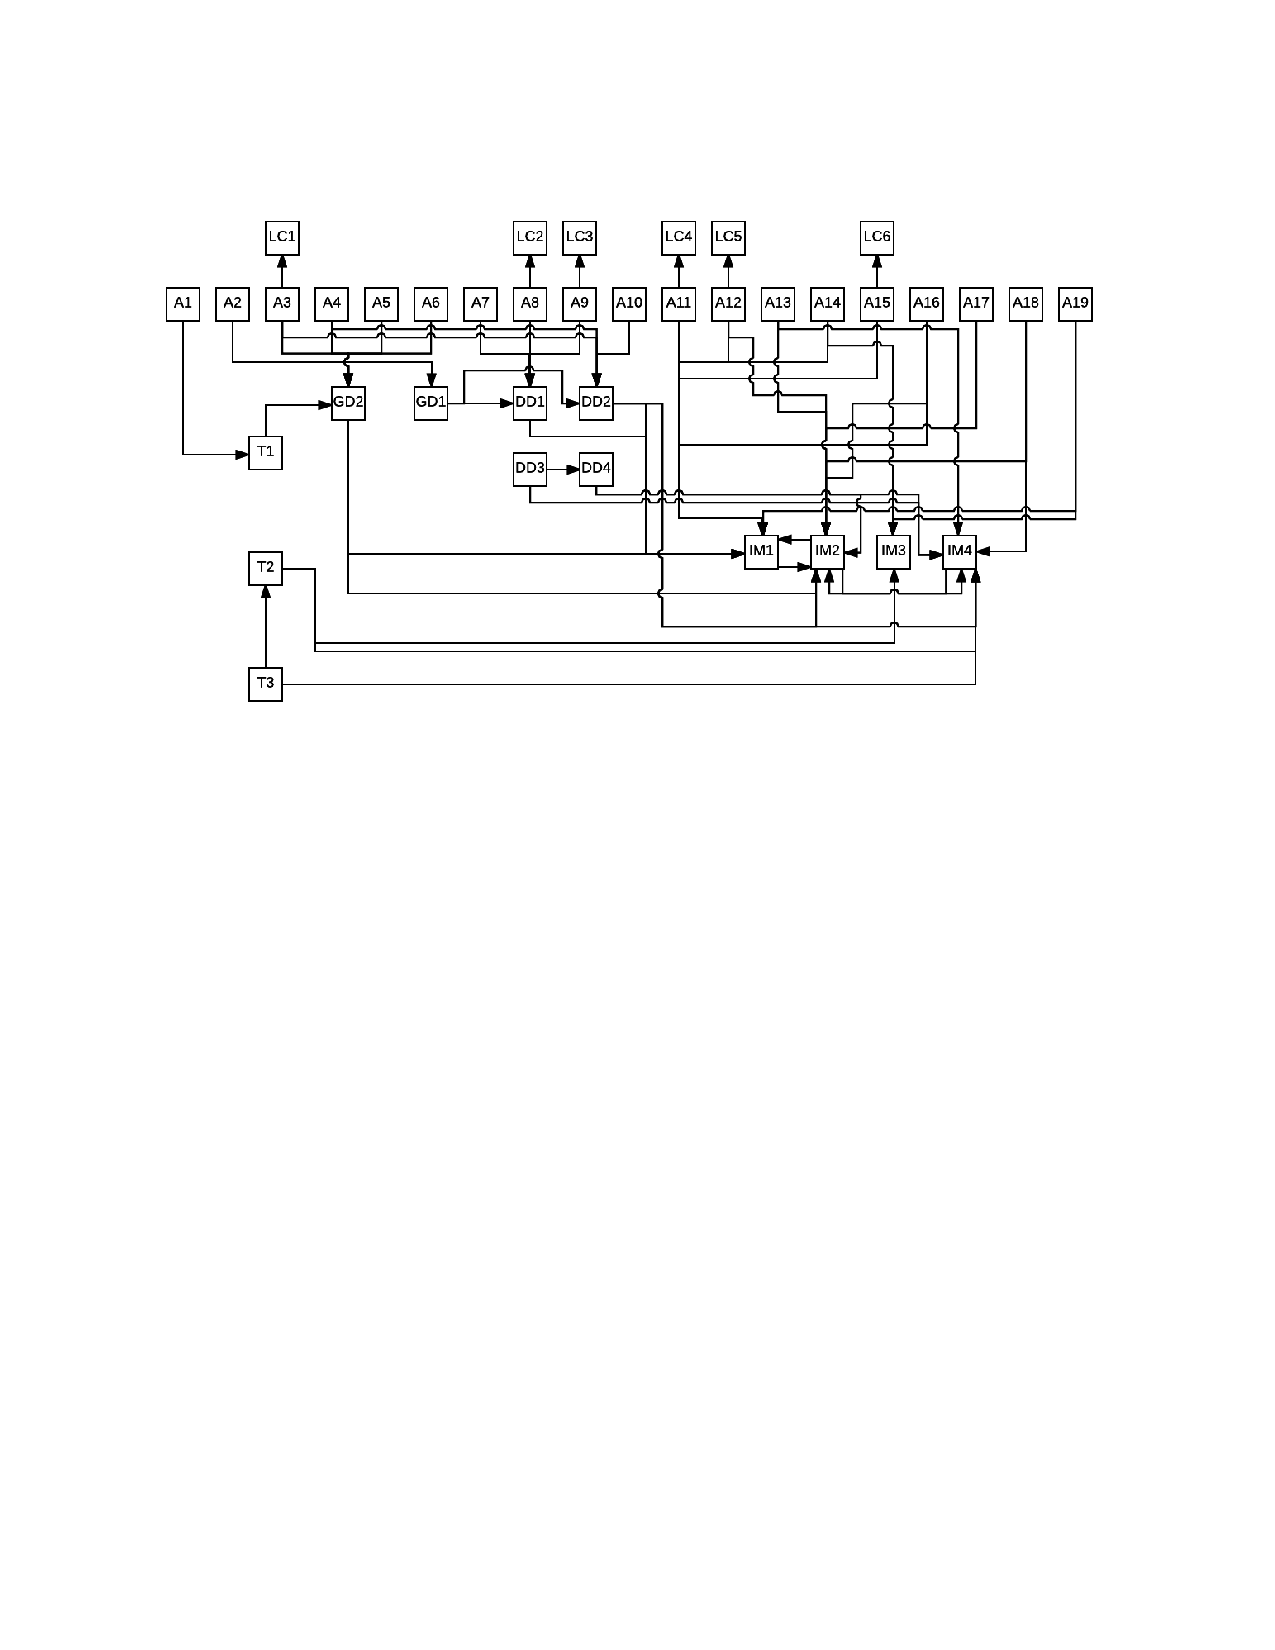
\includegraphics[scale=0.7]{../Figures/TraceGraph.pdf}
\end{center}

\end{frame}
%\hoffset=0in

%%%%%%%%%%%%%%%%%%%%%%%%%%%%%%%%%%%%%%

%\section[Qualities]{Qualities}

%%%%%%%%%%%%%%%%%%%%%%%%%%%%%%%%%%%%%%

\begin{frame}

\frametitle{Maintainability}

\begin{itemize}

\item[A1:] The
  only form of energy that is relevant for this problem is thermal energy.  All
  other forms of energy, such as mechanical energy, are assumed to be
  negligible [T1].

\item[A2:] All heat transfer coefficients are constant over time [GD1].

\item[A3:] The water in
  the tank is fully mixed, so the temperature is the same throughout the entire
  tank [GD2, DD2].

\item[A4:] The PCM has the same temperature throughout [GD2, DD2, LC1].

\item[A5:] etc.

\end{itemize}

\end{frame}

%%%%%%%%%%%%%%%%%%%%%%%%%%%%%%%%%%%%%%

\begin{frame}

\frametitle{Verifiability}

\begin{table} 
\centering
%\caption{Constraints on quantities}
\begin{tabular}{c c r c } 
\toprule
\textbf{Var} & \textbf{Constraints} & \textbf{Typical Value} & \textbf{Uncertainty}\\ \midrule
$L$ & $L > 0$ & 1.5 m & 10\% \\ 
$\rho_P$ & $\rho_P > 0$	& 1007 kg/m$^3$	& 10\% \\
\bottomrule
\end{tabular}
\label{tab:pcm}
\end{table}

\begin{equation*}
E_W = \int_{0}^{t} h_C A_C (T_C - T_W(t)) dt - \int_{0}^{t} h_P A_P (T_W(t) - T_P(t)) dt
\end{equation*}

\begin{itemize}
\item \structure{If wrong, wrong everywhere}
\item Sanity checks captured and reused
\item Generate guards against invalid input
\item Generate test cases
\item Generate view suitable for inspection
\item Traceability for verification of change
\end{itemize}
\end{frame}

%%%%%%%%%%%%%%%%%%%%%%%%%%%%%%%%%%%%%%

\begin{frame}

\frametitle{Reusability}

\noindent
\begin{minipage}{\columnwidth}
\begin{tabular}{@{} p{\colAwidth}  p{\colBwidth}@{}}
\toprule
\textbf{Num.}& \textbf{T1} \\
\midrule
Label &\bf Conservation of energy\\
\midrule
Eq &  $-{\bf \nabla \cdot q} +q'''$ = $\rho C \frac{\partial T}{\partial t}$ \smallskip\\
\midrule
Descrip & The above equation gives the conservation of energy for time 
varying heat transfer in a material of specific heat capacity $C$ and density $\rho$,
where $\bf q$ is the thermal flux vector, $q'''$ is the volumetric heat
generation, $T$ is the temperature, $\nabla$ is the del operator and $t$ is the time.\\
\bottomrule
\end{tabular}
\end{minipage}

\end{frame}

%%%%%%%%%%%%%%%%%%%%%%%%%%%%%%%%%%%%%%

\begin{frame}

\frametitle{Reusability}

\begin{itemize}
\item De-embed knowledge
\item Reuse throughout document
\begin{itemize}
\item Units
\item Symbols
\item Descriptions
\item Traceability information
\end{itemize}
\item Reuse between documents
\begin{itemize}
\item SRS
\item MIS
\item Code
\item Test cases
\end{itemize}
\item Reuse between projects
\begin{itemize}
\item Knowledge reuse
\item A family of related models, or reuse of pieces
\item Conservation of thermal energy
\item Interpolation, Etc.
\end{itemize}
\end{itemize}
\end{frame}

%%%%%%%%%%%%%%%%%%%%%%%%%%%%%%%%%%%%%%

\begin{frame}

\frametitle{Reproducibility}

\begin{itemize}
\item Usual emphasis is on reproducing code execution
\item However, \cite{IonescuAndJansson2013} show reproducibility challenges due to
undocumented:
\begin{itemize}
\item Assumptions
\item Modifications
\item Hacks
\end{itemize}
\item Shouldn't it be easier to independently replicate the work of others?
\item Require theory, assumptions, equations, etc.
\item Drasil can potentially check for completeness and consistency
\end{itemize}

\end{frame}

%%%%%%%%%%%%%%%%%%%%%%%%%%%%%%%%%%%%%%

\begin{frame}[fragile]

\frametitle{Smith and Koothoor (2016) \cite{SmithAndKoothoor2016}}

\begin{align}
R_1^{\mathrm{code}} &= \frac{f}{8\pi k_{\mathrm{AV}}} + \frac{1}{2\pi r_f h_g} \\
 R_1^{\mathrm{manual}} & = \frac {f}{8 \pi k_{\mathrm{AV}}}+ \frac{1}{2\pi r_f h_g}+\frac{\tau_c}{4\pi r_f k_c}
\end{align}

%actually equiv is hg is replaced with hp in the manual equation, since hg
%includes hg and kc
 
\begin{itemize}
\item Uncovered 27 issues with the previous documentation
\begin{itemize}
\item Incompleteness ($R_{\mbox{gap}}$)
\item Inconsistency($r$, $r_0$, $h_g$)
\item Verifiability problems ($R_1$)
\item Lack of traceability (circuit analogy)
\end{itemize}
\item Advantages of proposed approach
\begin{itemize}
\item Abstract to concrete
\item Separation of concerns
%\item Table of Symbols, unique labels, cross-referencing, and consistency checks
\item Every equation, assumption, definition, model, derivation, source and
  traceability between them
%\item Checklist.
\end{itemize}
\end{itemize}

\end{frame}

%%%%%%%%%%%%%%%%%%%%%%%%%%%%%%%%%%%%%%

%\section[Future Work]{Future Work}

%%%%%%%%%%%%%%%%%%%%%%%%%%%%%%%%%%%%%%

\begin{frame}

\includegraphics[width=\textwidth]{../Figures/no_silver_bullet.jpg}
\end{frame}

%%%%%%%%%%%%%%%%%%%%%%%%%%%%%%%%%%%%%
%\hoffset=-.7in %removing side bar for these frames
\begin{frame}[plain]

\frametitle{Future Work}

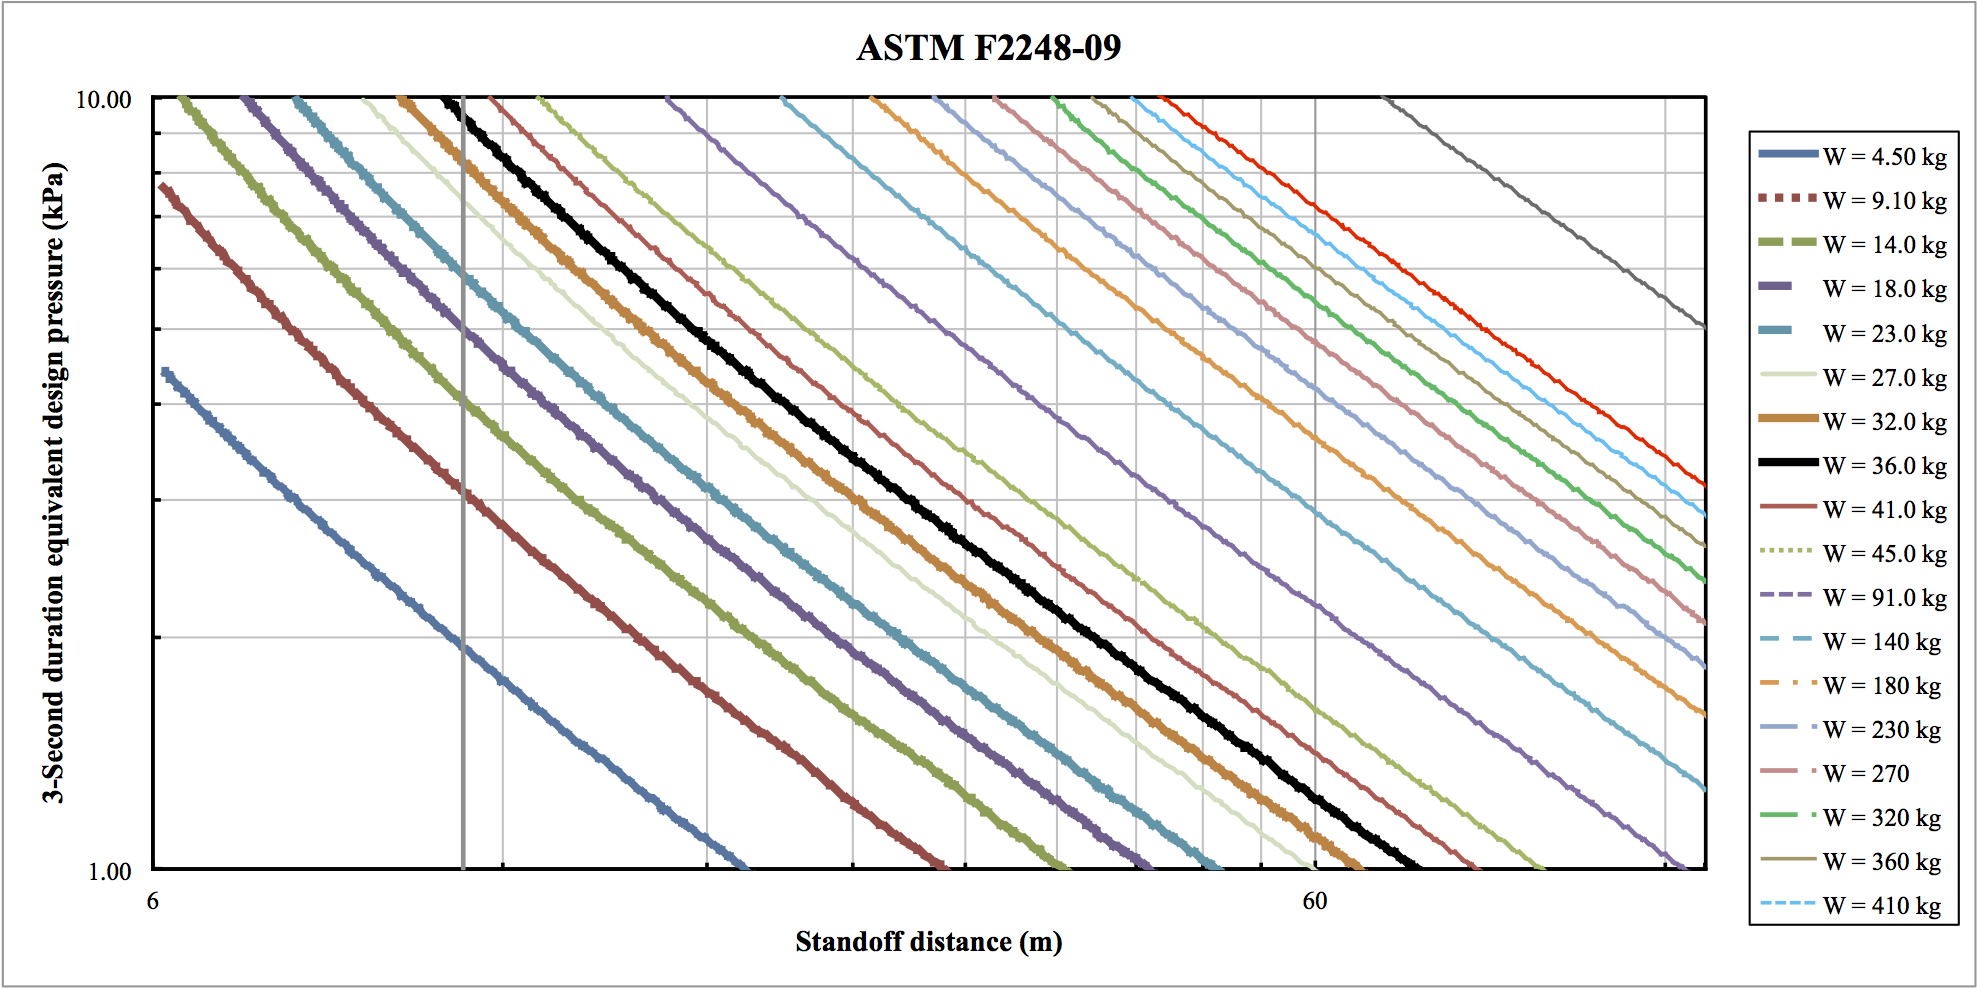
\includegraphics[width=1.\textwidth]{../Figures/ASTM_F2248-09.png}

\end{frame}
%\hoffset=0in %reset side bar for these frames
%%%%%%%%%%%%%%%%%%%%%%%%%%%%%%%%%%%%%%

%\section[Conclusions]{Conclusions}

%%%%%%%%%%%%%%%%%%%%%%%%%%%%%%%%%%%%%%

\begin{frame}

\frametitle{Drasil Framework for LSS}

\begin{itemize}
\item SCS has the opportunity to lead other software fields%  by leveraging its
  % solid existing knowledge base
\item Document driven design is feasible% with a knowledge-based approach
\item Requires an investment of time %to build knowledge base
\item Documentation does not have to be painful
\item Develop/refactor via practical case studies
\item Ontology may naturally emerge
\item Open source Drasil \href{https://github.com/JacquesCarette/literate-scientific-software}{here}
\end{itemize}


\includegraphics[width=0.5\textwidth]{../Figures/generate_all_the_things.jpg}

\begin{tikzpicture}[remember picture,overlay]
\node [xshift=2.75cm,yshift=-2.15cm] at (current page.center)
{
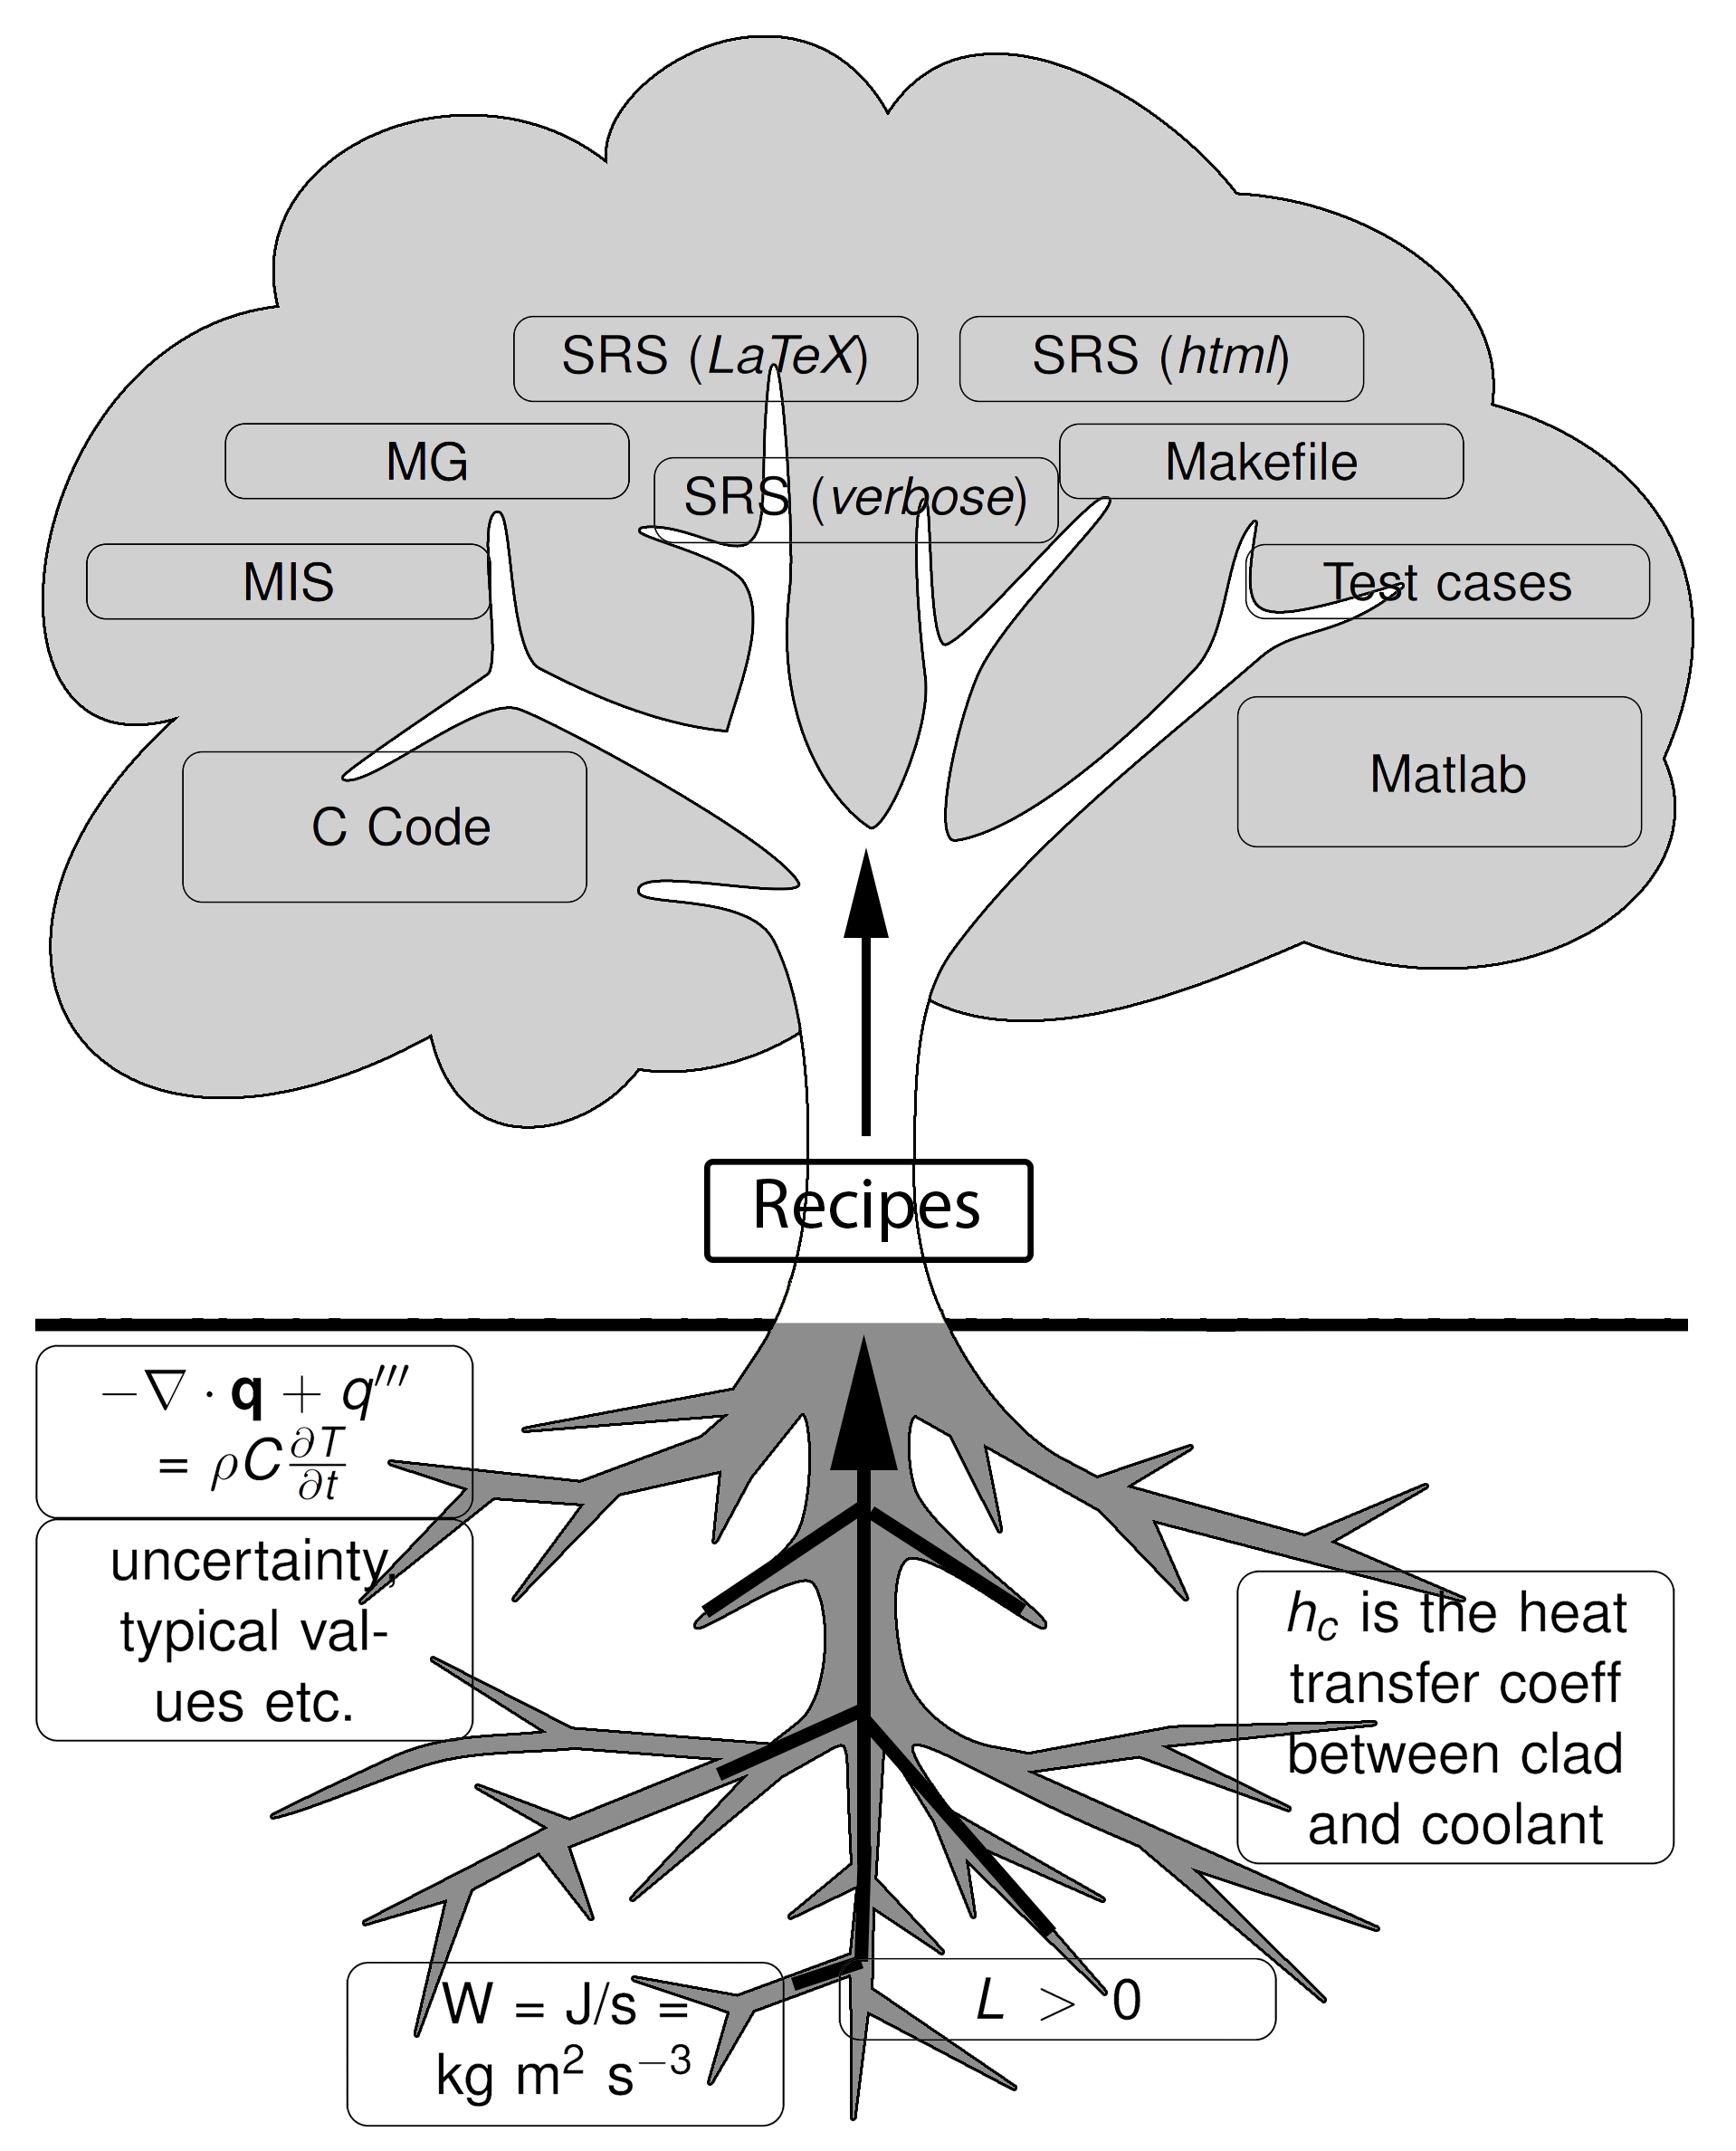
\includegraphics[height=10em]{../Figures/tree.png}
};
\end{tikzpicture}

\end{frame}

%%%%%%%%%%%%%%%%%%%%%%%%%%%%%%%%%%%%%%

\begin{frame}[allowframebreaks]
\frametitle{References}

\bibliography{../../ReferenceMaterial/References}

\end{frame}

%%%%%%%%%%%%%%%%%%%%%%%%%%%%%%%%%%%%%%%%%%%%%%%%%%%%%%

\end{document}